\documentclass[a4paper,twoside]{article}

\usepackage{epsfig}
\usepackage{subcaption}
\usepackage{calc}
\usepackage{amssymb}
\usepackage{amstext}
\usepackage{amsmath}
\usepackage{amsthm}
\usepackage{multicol}
\usepackage{balance}
\usepackage{pslatex}
\usepackage{apalike}
\usepackage{SCITEPRESS}     % Please add other packages that you may need BEFORE the SCITEPRESS.sty package.

\usepackage{microtype} % not included in scitepress

\usepackage{calc}
\usepackage{tikz}
\usetikzlibrary{calc,positioning,spy,shapes}


\tikzset{thick/.style = {line width = 1.0pt}}

\newlength{\pfull}  \setlength{\pfull}  {2mm}
\newlength{\phalf}  \setlength{\phalf}  {0.5\pfull}

\newlength{\lwffp}   \setlength{\lwffp}   {0.5000\dimexpr(\linewidth-1.0\pfull)}
\newlength{\lwfffp}  \setlength{\lwfffp}  {0.3333\dimexpr(\linewidth-2.0\pfull)}
\newlength{\lwffffp} \setlength{\lwffffp} {0.2500\dimexpr(\linewidth-3.0\pfull)}
\newlength{\lwfffffp}\setlength{\lwfffffp}{0.2000\dimexpr(\linewidth-4.0\pfull)}

\newlength{\twffp}   \setlength{\twffp}   {0.5000\dimexpr(\textwidth-1.0\pfull)}
\newlength{\twfffp}  \setlength{\twfffp}  {0.3333\dimexpr(\textwidth-2.0\pfull)}
\newlength{\twffffp} \setlength{\twffffp} {0.2500\dimexpr(\textwidth-3.0\pfull)}
\newlength{\twfffffp}\setlength{\twfffffp}{0.2000\dimexpr(\textwidth-4.0\pfull)}

\tikzstyle{labelStyle} = [ shape = rectangle, font = \scriptsize, text depth = 0, fill = white, inner sep = 4pt ]
\tikzstyle{labelN}  = [ labelStyle, anchor = north ]
\tikzstyle{labelNW} = [ labelStyle, anchor = north west ]
\tikzstyle{labelNE} = [ labelStyle, anchor = north east ]
\tikzstyle{labelS}  = [ labelStyle, anchor = south ]
\tikzstyle{labelSW} = [ labelStyle, anchor = south west ]
\tikzstyle{labelSE} = [ labelStyle, anchor = south east ]

\tikzstyle{figRC} = [shape = rectangle, rounded corners = 2mm, clip] % figure with Rounded Corners
\tikzstyle{spyRC} = [shape = rectangle, rounded corners = 2mm, %
    white, connect spies, every spy on node/.append style = {thick}] % spy with Rounded Corners
\tikzstyle{figNS} = [inner sep = 0pt, outer sep = 0pt] % figure with No Separators
 % includes tikz and calc, custom config by DL


\usepackage{url}
\usepackage[nolist]{acronym}
\usepackage[switch]{lineno}
\usepackage{hyperref}
\usepackage{cleveref}
\Crefname{figure}{Fig.}{Figs.}
\Crefname{table}{Tab.}{Tabs.}
\Crefname{equation}{Eqn.}{Eqns.}
\Crefname{algorithm}{Algo.}{Algos.}
\Crefname{section}{Sec.}{Secs.}
\usepackage[super]{nth}
\usepackage{csquotes}
\usepackage{wrapfig}
\usepackage{xcolor}
\usepackage[binary-units=true]{siunitx}

\usepackage{xspace}
\newcommand{\etal}{\textit{et~al}.\xspace}
\newcommand{\eg}{e.g.,\xspace} 
\newcommand{\ie}{i.e.,\xspace} 
\newcommand{\cf}{c.f.\xspace} 
\newcommand{\etc}{etc.\xspace} 
\newcommand{\vs}{vs.\xspace}


\begin{document}

\title{A Non-Photorealistic Rendering Technique\\for Art-directed Hatching of 3D Point Clouds}

\author{\authorname{%
    Ronja Wagner, %
    Ole Wegen~\orcidAuthor{0000-0002-6571-5897}, %
    Daniel Limberger~\orcidAuthor{0000-0002-9111-4809}, %
    J\"urgen D\"ollner, %
    and Matthias Trapp~\orcidAuthor{0000-0003-3861-5759}}
\affiliation{Hasso Plattner Institute, Faculty of Digital Engineering, University of Potsdam, Germany}
\email{\{ronja.wagner, ole.wegen\}@student.hpi.de, \{daniel.limberger, juergen.doellner, matthias.trapp\}@hpi.uni-potsdam.de}
}

\keywords{3D Point Clouds, Non-photorealistic Rendering, Real-time Rendering, Art-directed}

\abstract{%
    %
    Point clouds or point-based geometry of varying density can nowadays be easily acquired using \acs{LiDAR} cameras or modern smartphones with \acs{LiDAR} sensors.
    We demonstrate how this data can be used directly to create novel artistic digital content using \acl{NPR} techniques.
    We introduce a \acs{GPU}-based technique for art-directable \acs{NPR} rendering of 3D point clouds at interactive frame-rates.
    The technique uses either a subset or all of the points to generate oriented, sketchy strokes by taking local curvature and normal information into account.
    It uses X-Toon textures as part of its parameterization, supports hatching and cross hatching, and is inherently temporal coherent with respect to virtual camera movements.
    This introduces significant artistic freedom that is underlined by our results, which show that a variety of different sketchy styles such as colored crayons, pencil, pointillism, wax crayons, blue print, and chalk-drawings can be achieved on a wide spectrum of point clouds, i.e., covering 3D polygonal meshes as well as iPad-based LiDAR scans.
    %
}

\onecolumn \maketitle \normalsize \setcounter{footnote}{0} \vfill




\section{\texorpdfstring{\uppercase{Introduction}}{Introduction}}
\label{PCNPR:Sec:Introduction}
%
Point clouds are a simple, compact, and flexible geometric representation that can easily be acquired for real-world scenes using off-the-shelf photogrammetric techniques. 
With the introduction of \ac{LiDAR} sensors in high-end smartphones, \eg iPhone 12, straightforward acquisition of point clouds is easily accessible to consumers. 

\begin{figure}[t] % requires figures-spec.tex
    %
    \begin{tikzpicture}[figNS, spy using outlines = {style = spyRC, magnification = 3.0, size = 18mm}]
        % graphics:
        \node[figRC, anchor = south east](fig0) at (-\phalf,+\phalf)
            {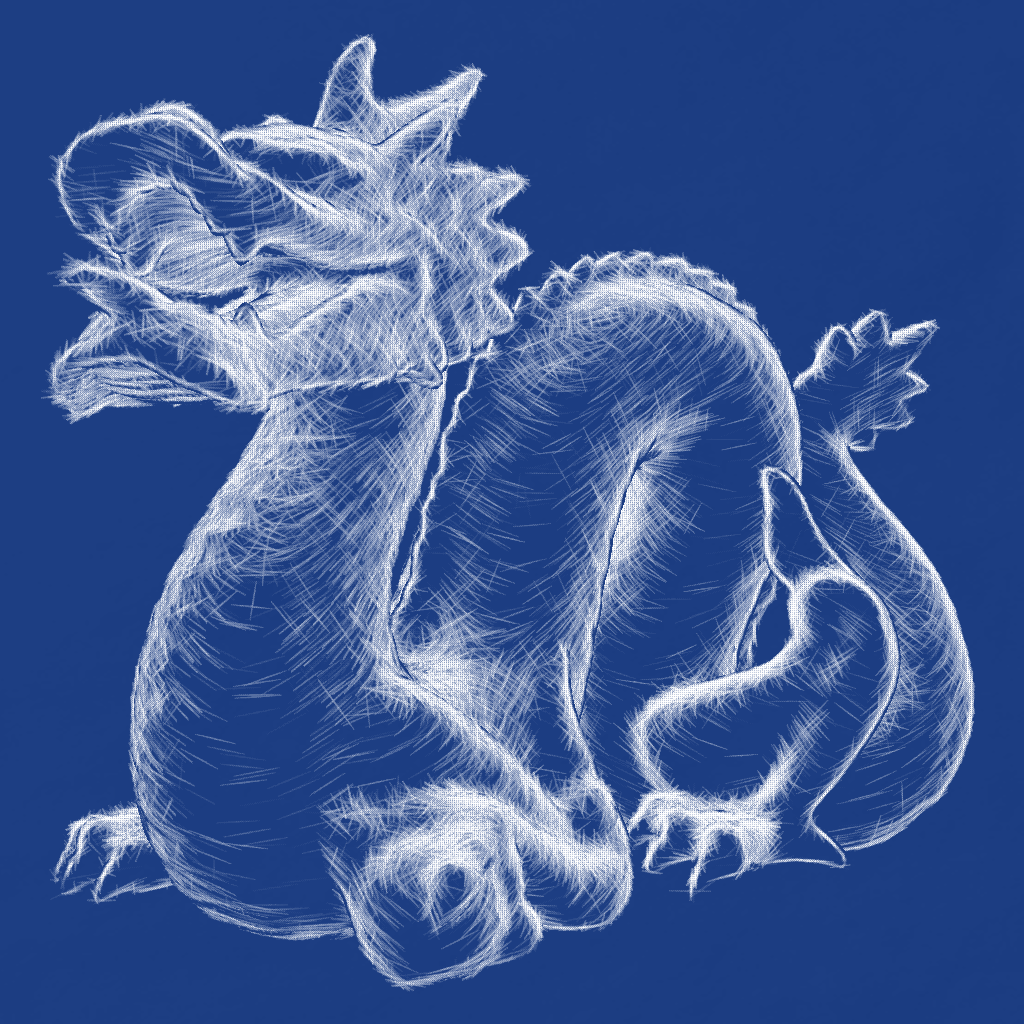
\includegraphics[width = \lwffp]{figures/dragon-blueprint-v2}};
        \node[figRC, anchor = south west](fig1) at (+\phalf,+\phalf)
            {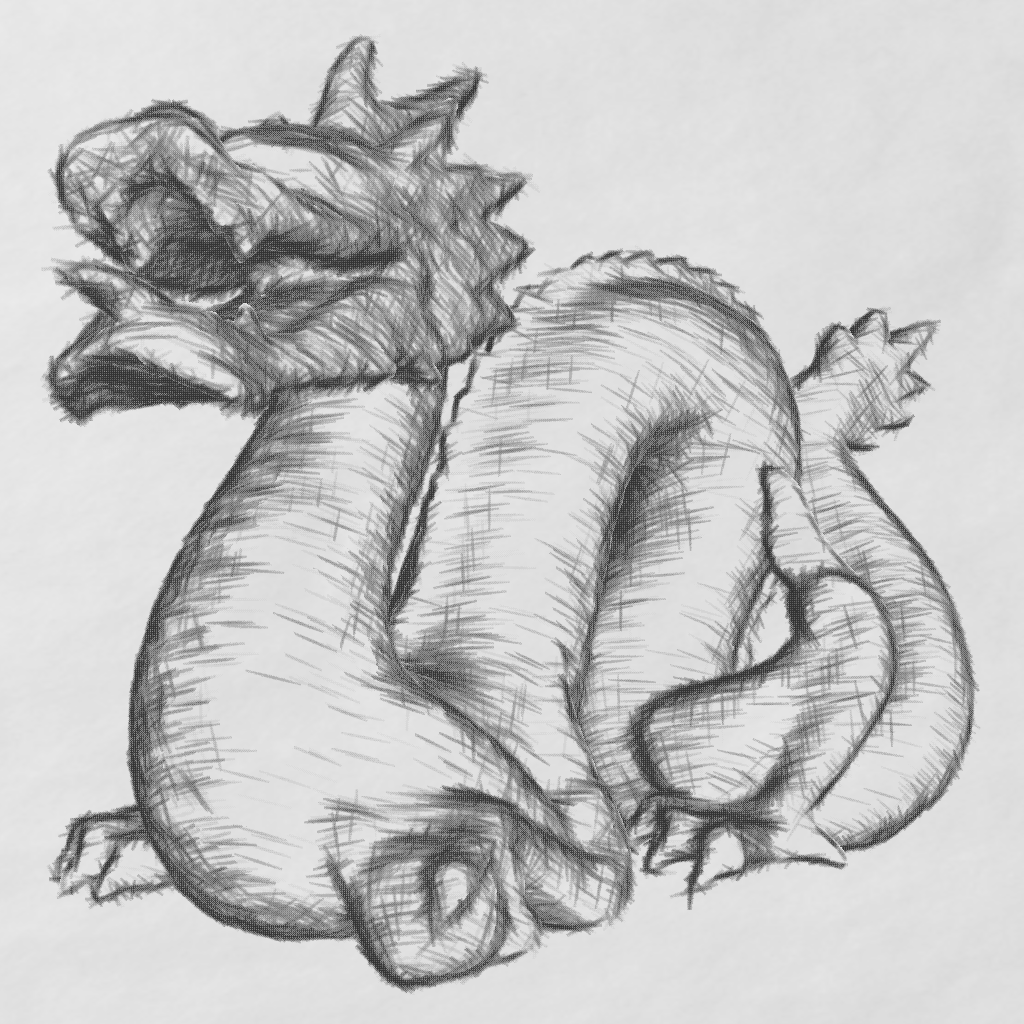
\includegraphics[width = \lwffp]{figures/dragon-pencil-v2}};
        \node[figRC, anchor = north east](fig2) at (-\phalf,-\phalf)
            {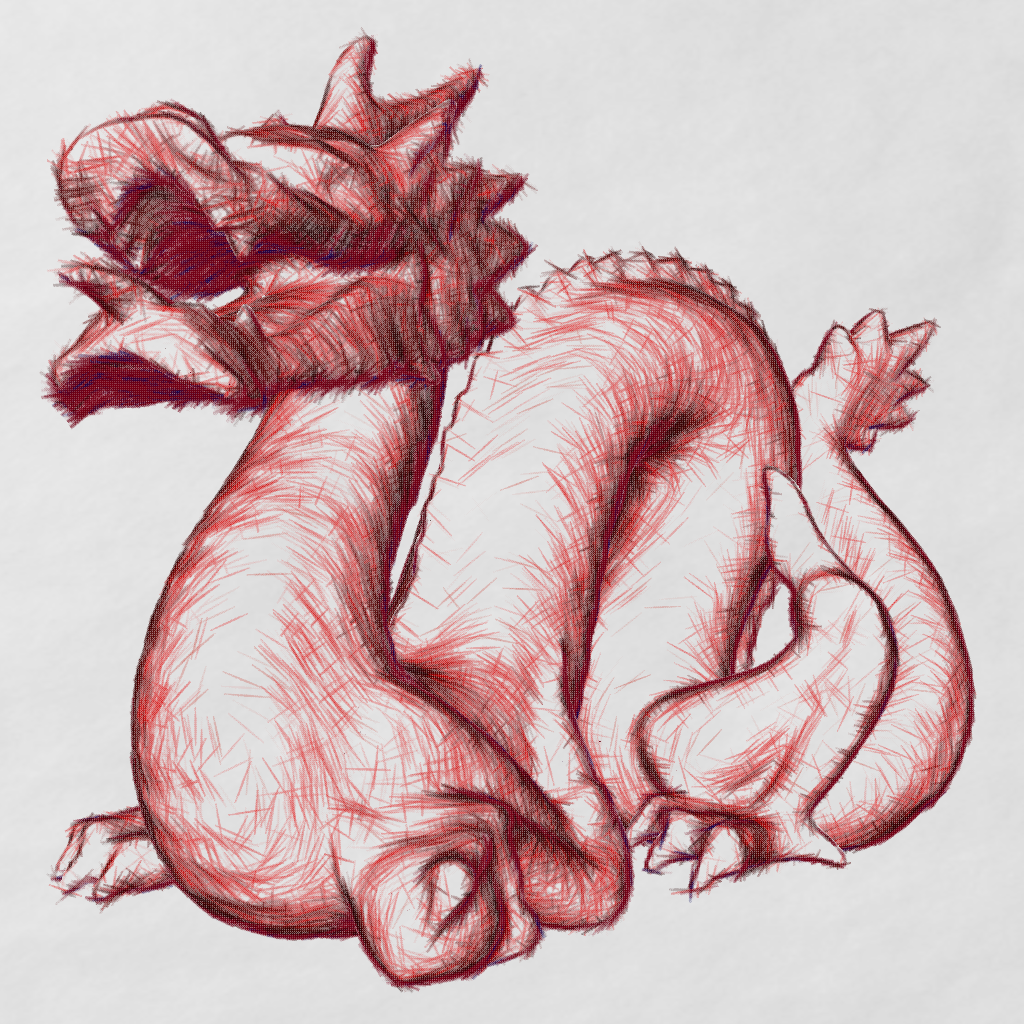
\includegraphics[width = \lwffp]{figures/dragon-multi-color-v2}};
        \node[figRC, anchor = north west](fig3) at (+\phalf,-\phalf)
            {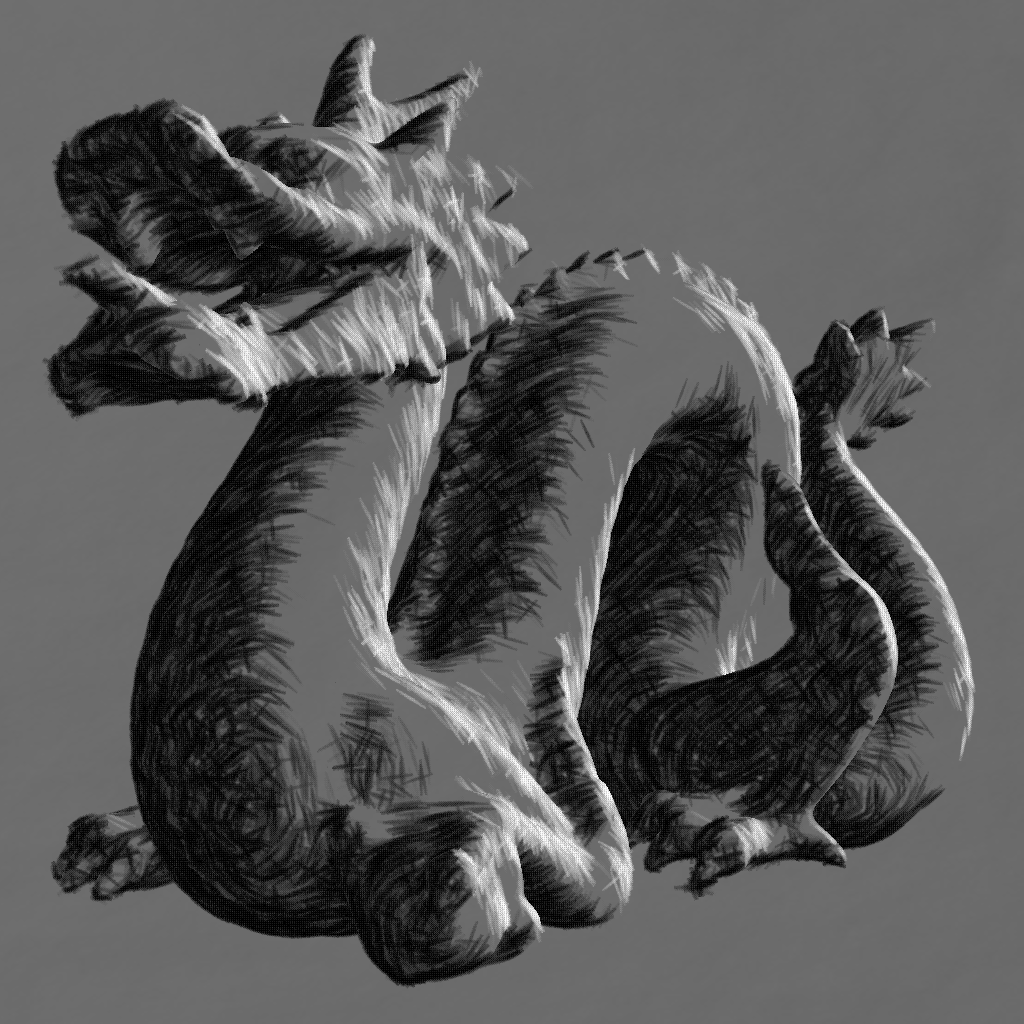
\includegraphics[width = \lwffp]{figures/dragon-wax-crayons-v2}};
        % sub-captions/labels:
        \node[above right = 0 of fig0, labelNE](lab0){(a)~Blue Print};
        \node[above right = 0 of fig1, labelNE](lab1){(b)~Pencil};
        \node[below left  = 0 of fig2, labelSW](lab2){(c)~Colored Crayons};
        \node[below left  = 0 of fig3, labelSW](lab3){(d)~Wax Crayons};
        % spies:
        \spy on ($(fig2.center)+(-9mm, +8mm)$) in node at ($(fig2.north)+(+7mm,-1mm)$);
        \spy on ($(fig3.center)+(-9mm, +8mm)$) in node at ($(fig3.north)+(+7mm,-1mm)$);
    \end{tikzpicture}
    %
    \caption{The \emph{Stanford dragon} as 3D point cloud, rendered in four different styles using art-direct hatching.}
    \label{PCNPR:Fig:Teaser}
\end{figure}
  
Despite both its potential applicability in various domains and increasing popularity in social media---mainly for 3D photography and animation with the point cloud as an art style in itself---%
their usage as a fundamental geometric representation in \ac{NPR} as well as respective rendering systems or frameworks are sparsely studied. Notable uses of 3D point clouds are 
  (1) to enable light transport for rendering scanned assets~\cite{Sabbadin2019}, 
  (2) stylized, interactive self portraits, 
  (3) data visualization, as well as
  (4) art-directed particle animation and stylization such as the reprojection of recorded memories in the computer game Cyberpunk 2077~\cite{ankermann2021} as a means of distinguishing between reality and virtual reality.
Another noteworthy use can be found in previsualization or digital content creation to evaluate ideas and concepts early before performing possibly costly data enhancement or transformation, \eg creating stylized, textured 3D meshes.
We present a first approach into this domain by researching methods to enable art-directed procedural-controlled rendering effects.

In the context of \ac{NPR}, point clouds have both advantages and disadvantages over traditional 3D polygonal models.
Point clouds lack inherent connectivity information that needs to be respected or maintained, which simplifies their representation, transformation, and rendering.
The absence of surface-related attributes such as normal vectors, texture coordinates, or curvature data is rather inconvenient, since they are essential for the implementation of \ac{NPR} techniques.
Additionally, while high quality renderings of point clouds are possible~\cite{Schuetz2015,Schuetz2021}, they often rely on a sufficient point density.
With these observations in mind, enabling the implementation of real-time, art-directed \ac{NPR} techniques comprises the following major challenges:

\begin{description}
    %
    \item[Art-directable Parametrization ($C_1$):] 
        Decoupling of processing operations that are required for different manifestations of stylization techniques, \eg point-splat functions \cite{Anjos2018}, to facilitate the interchange of respective techniques and increasing ease-of-use.
    %
    \item[Efficient Data Handling ($C_2$):] 
        An efficient representation of complex point clouds and respective stylization data to allow for art-directed stylization based on point-attribute data. This also concerns the reduction of data transfer and update latency to support real-time rendering for interactive control.
    %
\end{description}

Existing approaches to implement animation techniques for point clouds are
  (1) customized integration into existing game engines (to enable real-time rendering) or 
  (2) specific tooling or scripts to extend existing software, \eg Blender.
These, however, either require auxiliary constructs for data representation, \eg texture-based representations, lack real-time rendering capabilities, or can hardly handle millions of points.


In the context of the challenges $C_1$ and $C_2$, we present a \ac{GPU}-based hatching technique
for producing art-directed non-photorealistic renderings of potentially massive point clouds, which  
are obtained either using \ac{LiDAR} scanning of a real-world scene or by sampling polygonal geometry.
The presented approach is not limited to hatching, but can serve as a general approach for the implementation of further non-photorealistic rendering techniques for point clouds.

To this end, we\ldots
%
\begin{enumerate}
    \item \ldots{}introduce a method for creating sketched images directly out of 3D point clouds using only position, normal, and curvature information,
    \item enable significant artistic freedom due to wide range of parameters by using X-Toon textures, and
    \item demonstrate the method's real-time capability (precomputed attributes) and temporal coherence.
\end{enumerate}




\section{\texorpdfstring{\uppercase{Related Work}}{Related Work}}
\label{PCNPR:Sec:RelatedWork}
%
Prior art with respect to texture-based stylization in 3D object space using, \eg proxy-geometry as well as in image space remains quite popular and is well covered.
In the following, we briefly classify an exemplary cross section of classics as well as latest works.

\Ac{NPR} rendering of 3D polygonal meshes targeting a sketched look and feel can be easily achieved using texture-based hatching approaches~\cite{Praun2001,Webb2002}.
Hatching patterns are pre-generated in multiple levels of details, \ie \emph{Tonal Art Maps}, and enable fine control over shading without aliasing.
In order to also create sketchy outlines or silhouettes, image-based approaches can be applied~\cite{Nienhaus2003,Zakaria2004}.
These types of techniques, however, cannot be applied to point clouds, since texturing and image-based post processing is implemented fundamentally different; Strokes are placed directly and individually, and require a dedicated level of detail concept.
In addition, image-based curvature estimates~\cite{Kim2008} and purely image-based stippling~\cite{Awano2010} are not applicable and, regardless, usually lead to temporal incoherent results.

Another common approach for simulating, \eg pencil-like renderings, is to use edges of the 3D meshes to create overlapping graphite strokes~\cite{Sousa1999}.
This concept of creating textured proxy geometry, also sometimes referred to as graphtals~\cite{Smith1984}, facilitates temporal frame-to-frame coherence and can be applied to particles and point clouds alike~\cite{Kaplan2000,Markosian2000}.
The proxy geometry, \eg dots or strokes, can be specialized dynamically at run-time w.r.t. size, orientation, placement, and color.
Thereby, artistic control can be linked to mesh properties and thus allow for silhouettes and contouring~\cite{Grabli2004}.
This approach represents the core of our technique and, apart from various differences in the implementation details due to the evolution of graphic hardware, can be easily extend, enhanced, and specialized for point clouds.

A promising extension to this are \emph{ribbons}, \ie one-dimensional strips of points, ordered \enquote{according to their neighbourhood relations}~\cite{Runions2007}.
The concept could be used to create silhouette or curvature aware proxy geometry~\cite{Schmid2011} such as strokes consisting of multiple links instead of single, straight ones, and might allow for fine-grained stippling styles. 
So far, existing approaches covering water color, caligraphy, etc. still rely on strokes drawn by the artist~\cite{Zheng2017}.
Automatic splatting of lines or strokes, though applicable to volumetric data as well, does only cover a specific style and is not easily art-directable~\cite{Zhang2014,Anjos2018}.
We partially combine these ideas and aim for an automated approach that allows for a constrained but artist-directable, expressive stylization.




\section{\texorpdfstring{\uppercase{Art-directed Hatching}}{Art-Directed Hatching}}
\label{PCNPR:Sec:ArtDirectedHatching}
%
This section details concepts as well as implementation details of our real-time hatching technique.

\begin{figure}[t] % requires figures-spec.tex
    %
    \begin{tikzpicture}[figNS] %
        % graphics:
        \node[figRC, anchor = east](fig0) at (0,0)
            {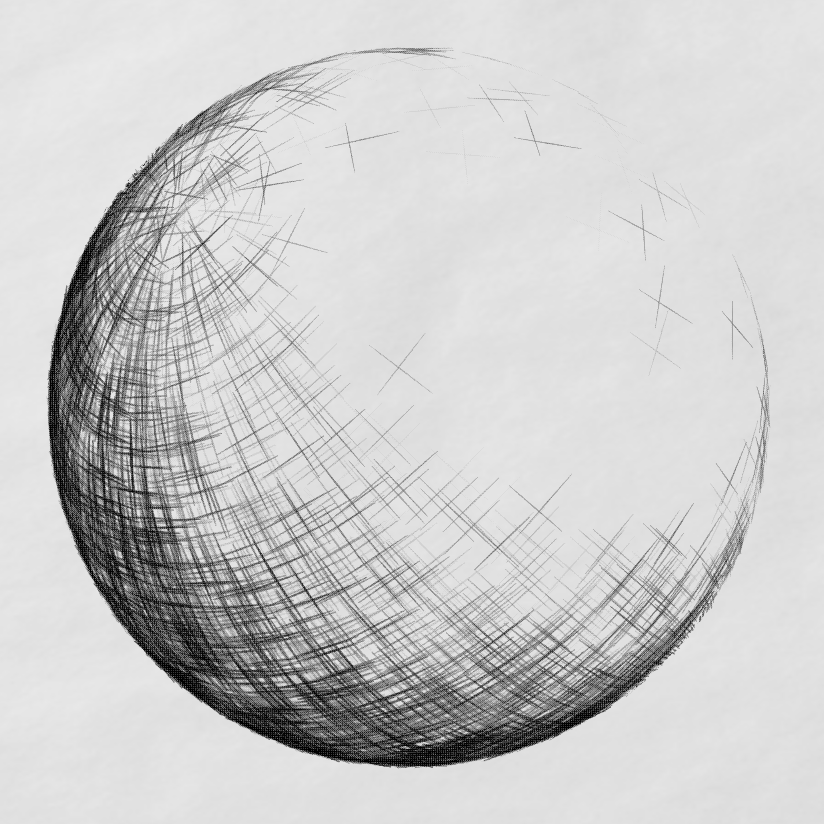
\includegraphics[width = \lwfffp - 0.25\pfull]{figures/xtoon-result-0}};
        \node[figRC, anchor = west](fig1) at ([xshift = \pfull] fig0.east) 
            {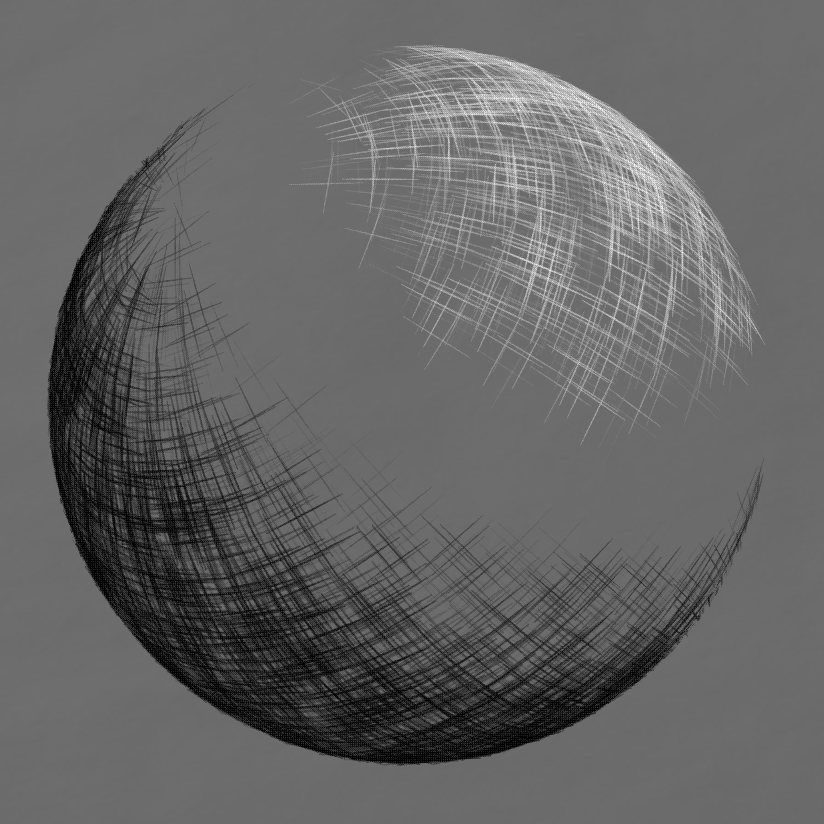
\includegraphics[width = \lwfffp - 0.25\pfull]{figures/xtoon-result-1}};
        \node[figRC, anchor = west](fig2) at ([xshift = \pfull] fig1.east) 
            {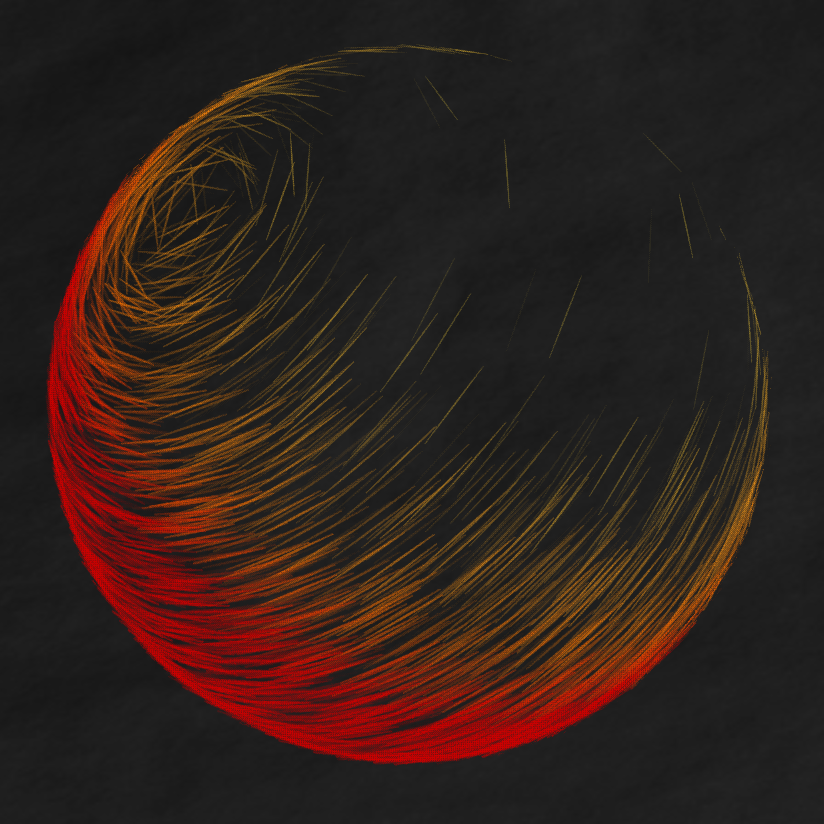
\includegraphics[width = \lwfffp - 0.25\pfull]{figures/xtoon-result-2}};
        % sub-figures
        \node[ultra thick, draw = white, anchor = north west](fig0m) at ([xshift = -0.75\pfull, yshift = -\pfull] fig0.north west) 
            {
\includegraphics[width = 0.3333\lwfffp]{figures/xtoon-map-0}};
        \node[ultra thick, draw = white, anchor = north west](fig1m) at ([xshift = -0.75\pfull, yshift = -\pfull] fig1.north west) 
            {
\includegraphics[width = 0.3333\lwfffp]{figures/xtoon-map-1}};
        \node[ultra thick, draw = white, anchor = north west](fig2m) at ([xshift = -0.75\pfull, yshift = -\pfull] fig2.north west) 
            {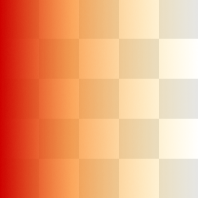
\includegraphics[width = 0.3333\lwfffp]{figures/xtoon-map-2}};
        % sub-captions/labels:
        \node[below = 0 and -1mm of fig0, labelN](lab0){(a)~Pencil.};
        \node[below = 0 and -1mm of fig1, labelN](lab1){(b)~Wax crayon.};
        \node[below = 0 and -1mm of fig2, labelN](lab2){(c)~Two-colored.};
        % spies:
    \end{tikzpicture}
    %
    \caption{Shading effects and their corresponding X-Toon textures (RGBA). 
        Note that the y-axis is not utilized here.}
    \label{PCNPR:Fig:XToon}
    %
\end{figure}



\subsection{Art-Directed Parametrization}
\label{PCNPR:SubSec:ConceptualOverview}
%
We make the assumption that any point cloud is given with point normal vectors~\cite{Cao2021}, color, and curvature attributes~\cite{Merigot2009,Lu2020}.
The latter two can improve the appearance but are not required.
To achieve the desired hatching effect, each point is replaced by textured proxy geometry, \eg two orthogonal lines aligned to the surface, textured with pencil strokes.

A drawing technique that characterizes cross-hatching is to depict lighting by not only using different colors but also by omitting lines and therefore showing the underlying paper.
The amount of light that reaches a point defines how likely it is to be omitted. 
To accomplish a wide variety of artistic styles and effects, the color and point density for each amount of light can be controlled through the alpha channel of an X-Toon~\cite{Barla2006,Kang2009} texture~(\Cref{PCNPR:Fig:XToon}).
On white paper for example, strongly illuminated parts are realized by removing most points, while darker parts keep their original point density.
Another option (better suited to darker backgrounds) is to color well-lit points brightly and leave out points receiving a medium amount of light.

Lighting by omission only works if there are no visible parts behind the points that are left out.
To avoid such parts, \eg the back of the model, from appearing where only the paper should be visible, we use an additional depth pass. With that pass we ensure that nothing behind the surface of the model is visible in the final result.

For a more realistic pencil effect there is also the option to limit the stroke colors to a number of pre-defined pencil colors, similar to a colored pencil set.
In addition to the classic X-Toon parametrization, the following parameters are provided for hatching:

\begin{description}
    %
    \item[Line Length and Thickness:] 
        These parameters control the extent of hatching strokes.
    %
    \item[Parallel to cross-hatch Proportion:] 
        Our technique supports both cross hatching, where almost all points are replaced with two lines, and parallel hatching, where all points are replaced with a single line. 
        This parameter specifies the probability for a point to be replaced with a single stroke or two, crossed strokes.
    %
    \item[Stroke Density:] 
        In point clouds of high density, the individual hatched strokes might not be distinguishable from each other. 
        By specifying the proportion of strokes to be left out, the density of rendered strokes can be controlled.
    %
    \item[Line Direction:] 
        This parameter is used to determine the direction of each stroke.
    %
    \item[Light Direction:]
        For lighting we use a uniform light direction that is specified by this parameter.
    %
    \item[Coloring Mode:] 
        Defines which method is to be used for determining the color of the hatched strokes.
    %
    \item[Hue Shift:] 
        Is applied to the color calculated with the selected coloring mode.
    %
\end{description}



\subsection{Stroke Generation for Hatching}
\label{PCNPR:SubSec:HatchStrokeGeneration}


\paragraph{X-Toon Coordinate Computation.}
%
To determine the desired density and therefore the proportion of points to be omitted, we first compute the X-Toon texture coordinates, namely depth and brightness, for a point.
Transforming the point's z-coordinate (after projection) into a $[0,1]$ range yields the depth coordinate. 
The brightness coordinate depends on the scene lighting implementation, e.g., Phong-based lighting~\cite{Phong1975}. 
With these coordinates and the corresponding texture value, we determine whether the current point should be discarded or replaced by lines, and in the latter case, obtain the color of these lines.


\paragraph{Probabilistic Interpolation.}
%
Both lighting by omission and the pencil color quantization rely on a probabilistic approach. 
Instead of interpolating between two values (\eg visible and not visible or two RGB values) and applying the result, the point only attains one of the values chosen at random with the interpolation factor determining the probabilities. 
With a sufficient number of points, the result creates an approximate impression of directly interpolated values.
As random seed, we use the point ID, which is temporally consistent.
For determining whether a point should be visible or not, we use the alpha value from the X-Toon texture as the interpolation factor between visibility and invisibility. 
So if $a\in [0;1]$ is the alpha value, the point has a $100\cdot a \%$\, chance of being visible.
The general point density can be controlled through a corresponding parameter that we multiply with the alpha value from the X-Toon texture.

\begin{figure}[t] % requires figures-spec.tex
    %
    \centering
    \begin{tikzpicture}[figNS] %
        % graphics:
        \node[figRC, anchor = east](fig0) at (0,0)
            {
\includegraphics[width = 0.8\lwffp]{figures/hatching-regular-v2}};
        \node[figRC, anchor = west](fig1) at ([xshift = \pfull] fig0.east) 
            {
\includegraphics[width = 0.8\lwffp]{figures/hatching-irregular-v2}};
        % sub-captions/labels:
        \node[below = 0 and -0.375\pfull of fig1, labelN](lab1){(b)~Irregular Stroke Placement};
        \node[below = 0 and -0.375\pfull of fig0, labelN](lab0){(a)~Regular Stroke Placement};
        % spies:
    \end{tikzpicture}
    %
    \caption{For hatching, one or more strokes, \ie two for cross-hatching, can be placed and oriented either in a (a)~regular more accurate or (b)~irregular and scattered way.}
    \label{PCNPR:Fig:Hatching}
    %
\end{figure}


\paragraph{Line Geometry Generation.}
%
For the cross hatching effect we replace each point with two orthogonal lines perpendicular to the point's normal.
In doing so, we need to ensure the line directions are consistent for all points.
Line directions are consistent if points with similar normal vectors produce similar line directions~(\Cref{PCNPR:Fig:Hatching}) so that they properly illustrate the surface direction.
To achieve that consistency we project a normalized uniform vector on the plane defined by each point normal.
%
Let $\vec u$ be the uniform vector and $\vec n$ be the surface normal. 
The projected vector $\vec d_1$ is computed as follows: $\vec d_1 = \vec u - (\vec u \cdot \vec n) \cdot \vec n$.
The second direction $\vec d_2$ can be determined by simply computing the normalized cross product of the first direction and the point normal: $\vec d_2 = \vec n \times \vec d_1$.
With these directions, we can now create two orthogonal lines along the surface. Let $p$ be the point coordinates and $l$ be the line length parameter. 
Then the first line extends from $p - \vec d_1$ to $p + \vec d_1$. The second line starts at $p - \vec d_2$ and ends at $p + \vec d_2$.
We can now use these coordinates to create rectangle geometry for each line. 
One side of said rectangle is described by the corresponding line direction and length. 
The direction of the other side needs to be orthogonal to both the line direction and the vector from the camera to the current point and can therefore be calculated by taking their cross product.
The width of the line is defined in a separate line thickness parameter. 
From this information, we can derive the four vertices of the resulting rectangle, with the texture coordinates $(0,0)$, $(0,1)$, $(1, 1)$ and $(1,0)$ for the pencil stroke texture.



\subsection{Local Shading Models}
\label{PCNPR:Sec:Colors}

There are three ways to determine the color of the created pencil strokes.
The simplest one is to apply the same color to all strokes, which can, for example, be used to create a classic gray pencil sketch or a blue ballpoint pen drawing. Alternatively, the color can be taken directly from the X-Toon texture. The third approach is to blend the initial point color with the X-Toon texture value to depict both lighting and the original color information.

After the point color is determined, it is possible to add pencil color quantization.
That means only allowing colors from a predefined set to simulate drawing with pencils from a limited pencil box.
Unlike other media, pencil colors can only be mixed to a limited extent.
With watercolors for example, three colors and black and white are in theory sufficient to get every other color.
For colored pencils however, you need more base colors to illustrate the whole color spectrum properly. This is because generally, the quality of the blending result of two pencil colors suffers with decreasing similarity of the blended colors.

Our pencil color effect simulates that by calculating the two closest colors from a predetermined pencil set to a given color and blending them with probabilistic interpolation.
We call the given color $c_0$. 
The pencil color set is given as rgb and hsv values sorted by hue. It contains only colors with high saturation and value.
First, we calculate the hsv representation of $c_0$ and apply the hue shift parameter.
We can then search for the colors $c_1$ and $c_2$ from the pencil set whose hues are closest to $c_0$'s hue, so that $\textrm{hue}(c_0) = \textrm{hue}(c_1)\cdot a + \textrm{hue}(c_2)\cdot (1-a)$ applies for an $a\in [0,1]$.
We can use this $a$ as an interpolation factor for probabilistic interpolation to create the impression of a color with the same hue as $c_0$.
Finally, we mix the resulting color with black and white to more closely match $c_0$ in value and saturation.

\begin{figure}[b] % requires figures-spec.tex
    %
    \begin{tikzpicture}[figNS] %
        % graphics:
        \node[figRC, anchor = east](fig0) at (0,0)
            {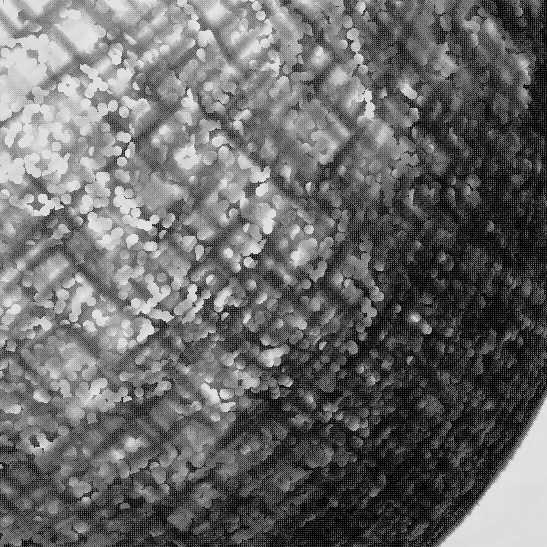
\includegraphics[width = \lwfffp, trim = 96 64 96 0, clip]{figures/polygon-offset-without-z-v2-crop}};
        \node[figRC, anchor = west](fig1) at ([xshift = \pfull] fig0.east) 
            {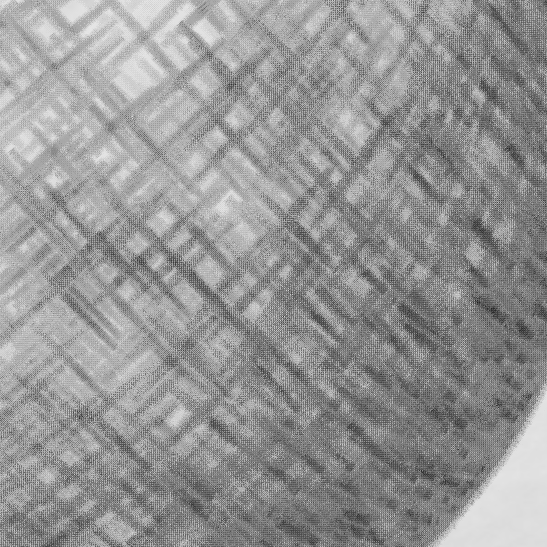
\includegraphics[width = \lwfffp, trim = 96 64 96 0, clip]{figures/no-depth-mask-v2-crop}};
        \node[figRC, anchor = west](fig2) at ([xshift = \pfull] fig1.east) 
            {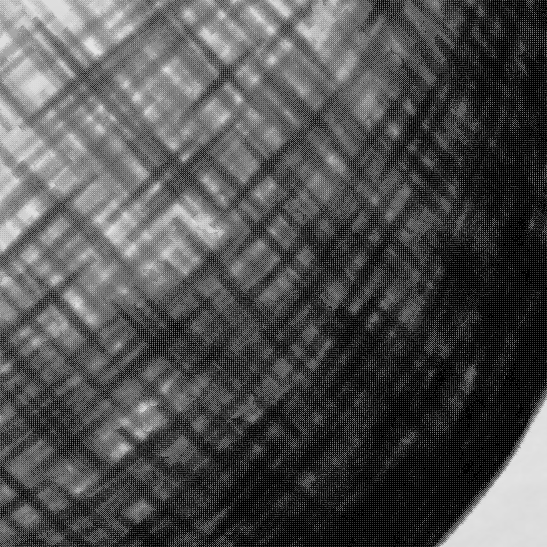
\includegraphics[width = \lwfffp, trim = 96 64 96 0, clip]{figures/polygon-offset-with-z-v2-crop}};
        % sub-captions/labels:
        \node[below left = 0 of fig0, labelSW](lab0){(a)};
        \node[below left = 0 of fig1, labelSW](lab1){(b)};
        \node[below left = 0 of fig2, labelSW](lab1){(c)};
        % spies:
    \end{tikzpicture}
    %
    \caption{%
        The point sprites used during the depth pass cause discontinuities in the z-buffer which interfere with the strokes rendered later~(a). 
        In addition, the semi-transparent strokes interfere with one another~(b). %
        By shifting the strokes towards the virtual camera using polygon offsets while using order-independent rendering (blending or alpha to coverage) both effects can be circumvented respectively~(c).}
    \label{PCNPR:Fig:PolygonOffset}
    %
\end{figure}

\begin{figure}[b] % requires figures-spec.tex
    %
    \begin{tikzpicture}[figNS] %
        % graphics:
        \node[figRC, anchor = east](fig0) at (0,0)
            {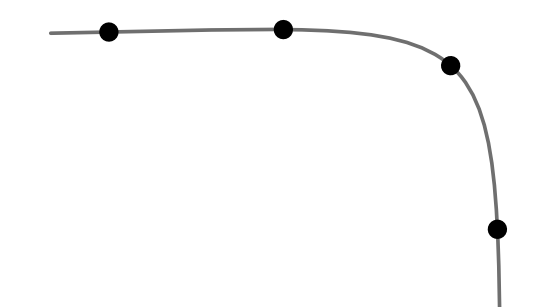
\includegraphics[width = \lwfffp]{figures/curvature1-v2}};
        \node[figRC, anchor = west](fig1) at ([xshift = \pfull] fig0.east) 
            {
\includegraphics[width = \lwfffp]{figures/curvature2-v2}};
        \node[figRC, anchor = west](fig2) at ([xshift = \pfull] fig1.east) 
            {
\includegraphics[width = \lwfffp]{figures/curvature3-v2}};
        % sub-captions/labels:
        \node[below = 0 and -0.375\pfull of fig0, labelN](lab0){(a)~Points};
        \node[below = 0 and -0.375\pfull of fig1, labelN](lab1){(b)~W/o  alignment};
        \node[below = 0 and -0.375\pfull of fig2, labelN](lab1){(c)~With alignment};
        % spies:
    \end{tikzpicture}
    %
    \caption{The length of strokes can be aligned based on the local curvature at the stroke's location.
        This can be used to achieve (b)~increased sketchiness especially in curved areas as well as (c)~a strict, more accurate hatching.}
    \label{PCNPR:Fig:Curvature}
    %
\end{figure}



\subsection{Depth Pass}
\label{PCNPR:SubSec:DepthPass}
%
For the lighting by omission approach to work, we need to ensure there are no visible lines behind the points that are omitted.
A first approach to that problem is back face culling, which prevents the back of the surface from being visible.
However, even with back face culling, there still are lines behind the surface that are not supposed to be visible~(\Cref{PCNPR:Fig:DepthPass}).
We prevent that by using an additional rendering pass before the hatching pass.

\begin{figure*}[t] % requires figures-spec.tex
    %
    \begin{tikzpicture}[figNS, spy using outlines = {style = spyRC, magnification = 2.5, size = 16mm}]
        % graphics:
        \node[figRC, anchor = east](fig0) at (0,0)
            {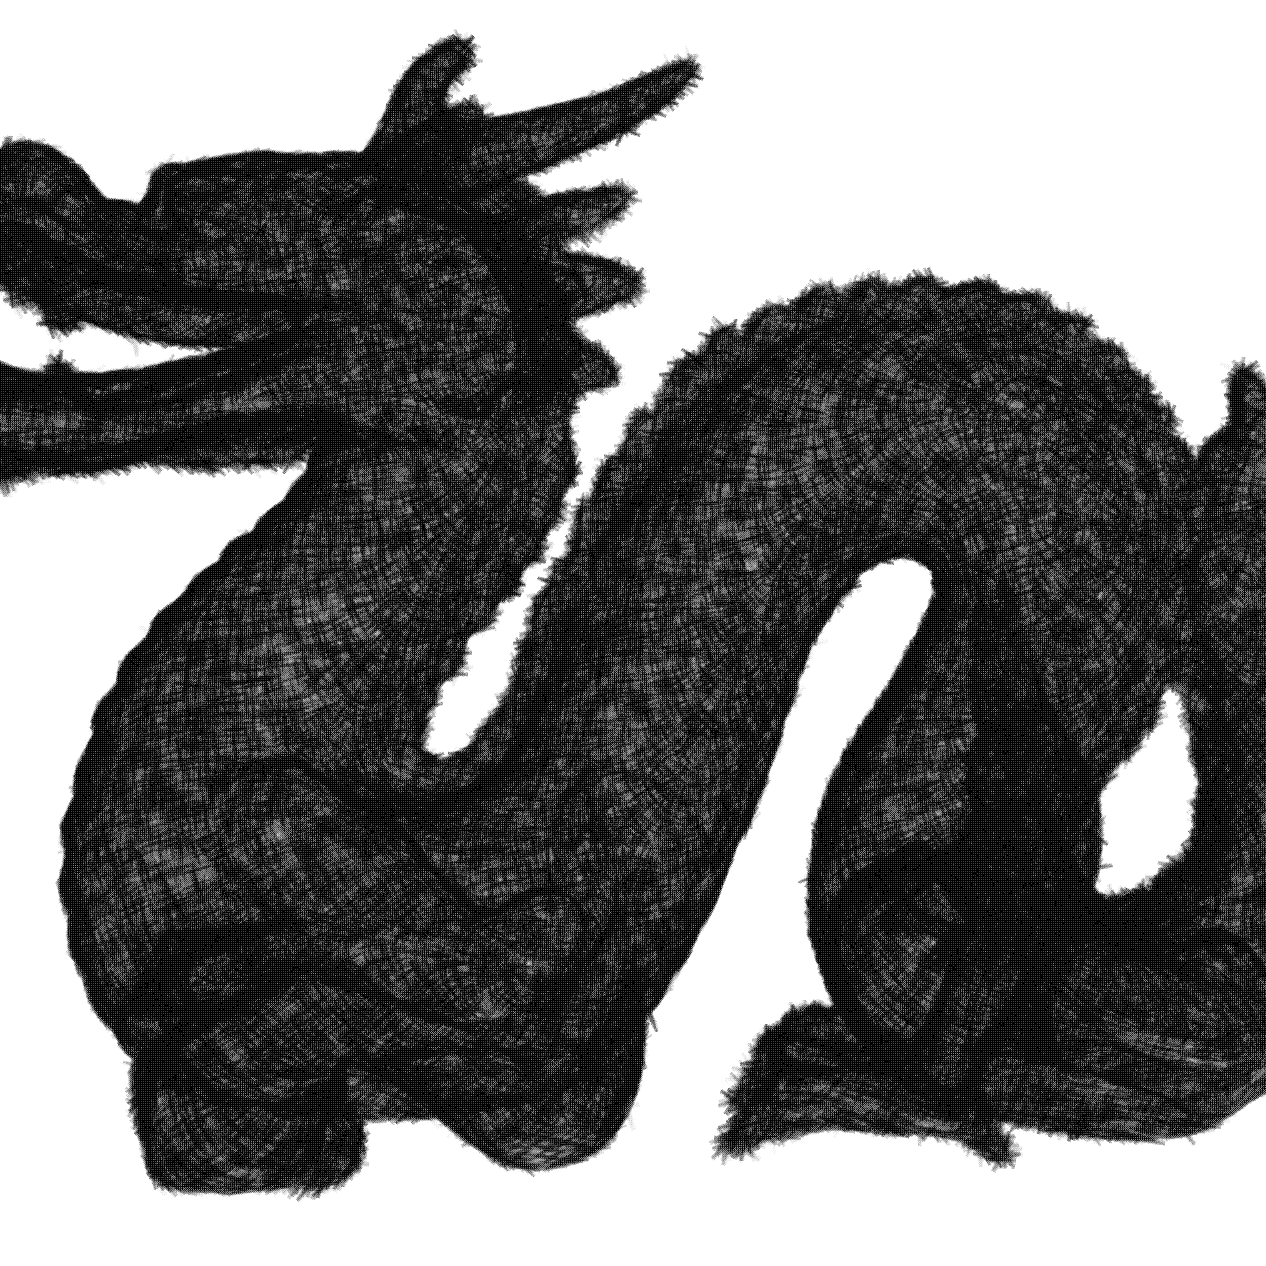
\includegraphics[width = \twffffp]{figures/dragon-no-culling-v2-square}};
        \node[figRC, anchor = west](fig1) at ([xshift = \pfull] fig0.east) 
            {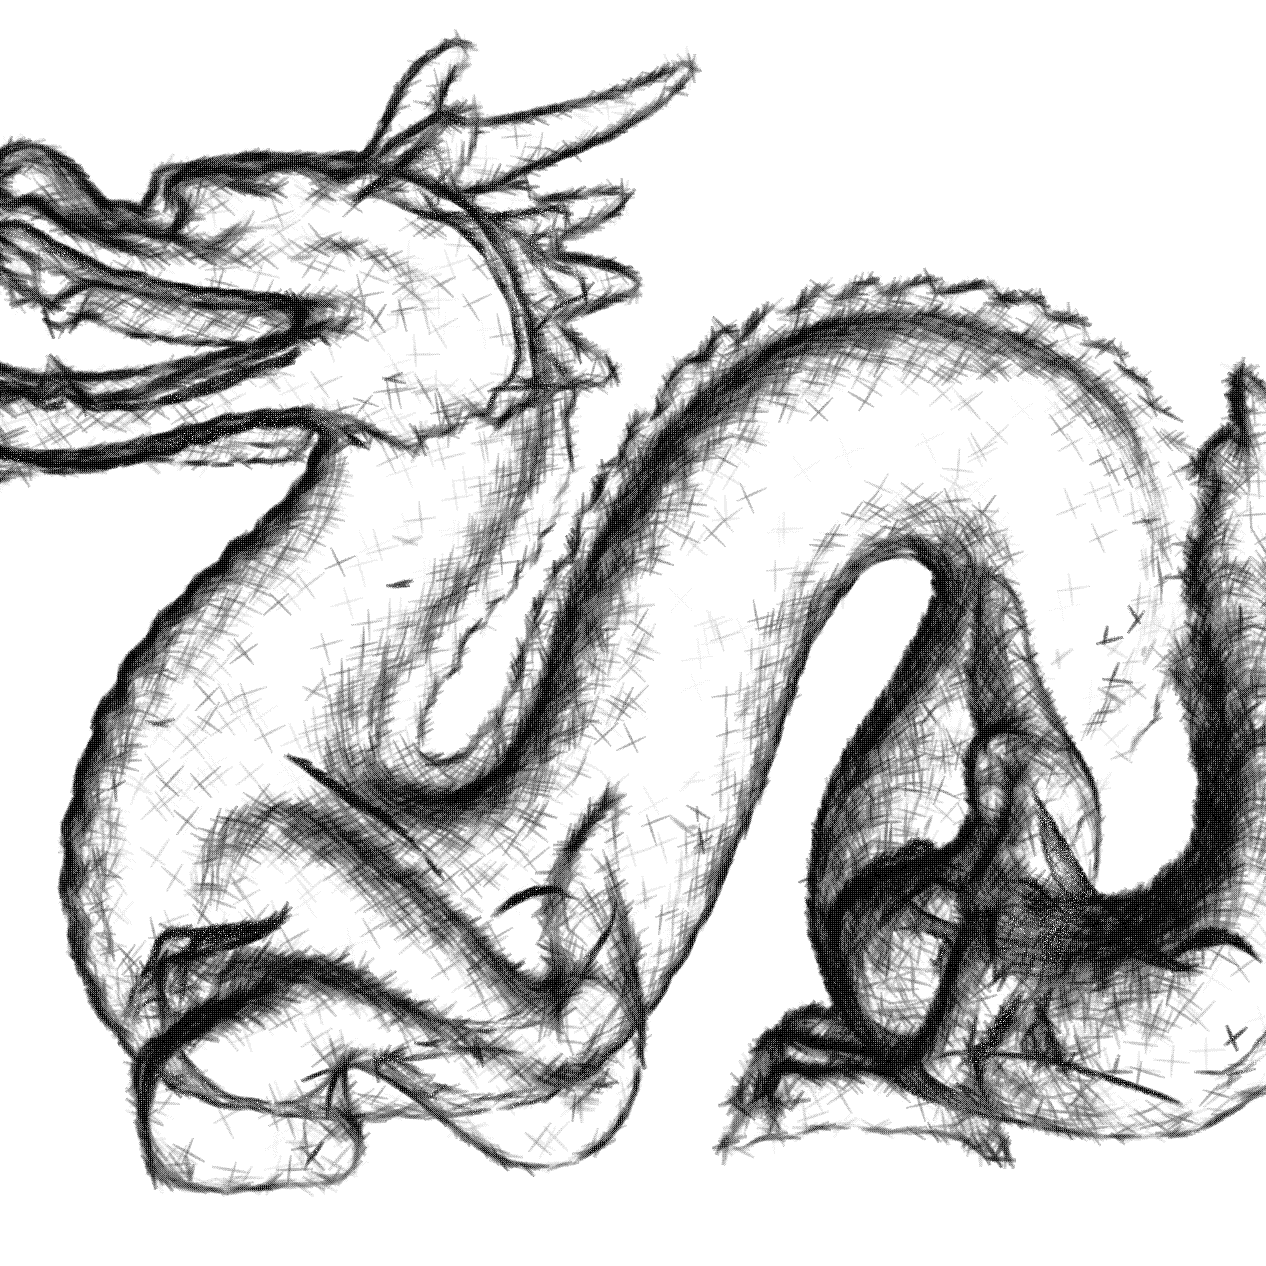
\includegraphics[width = \twffffp]{figures/dragon-no-depth-v2-square}};
        \node[figRC, anchor = west](fig2) at ([xshift = \pfull] fig1.east)
            {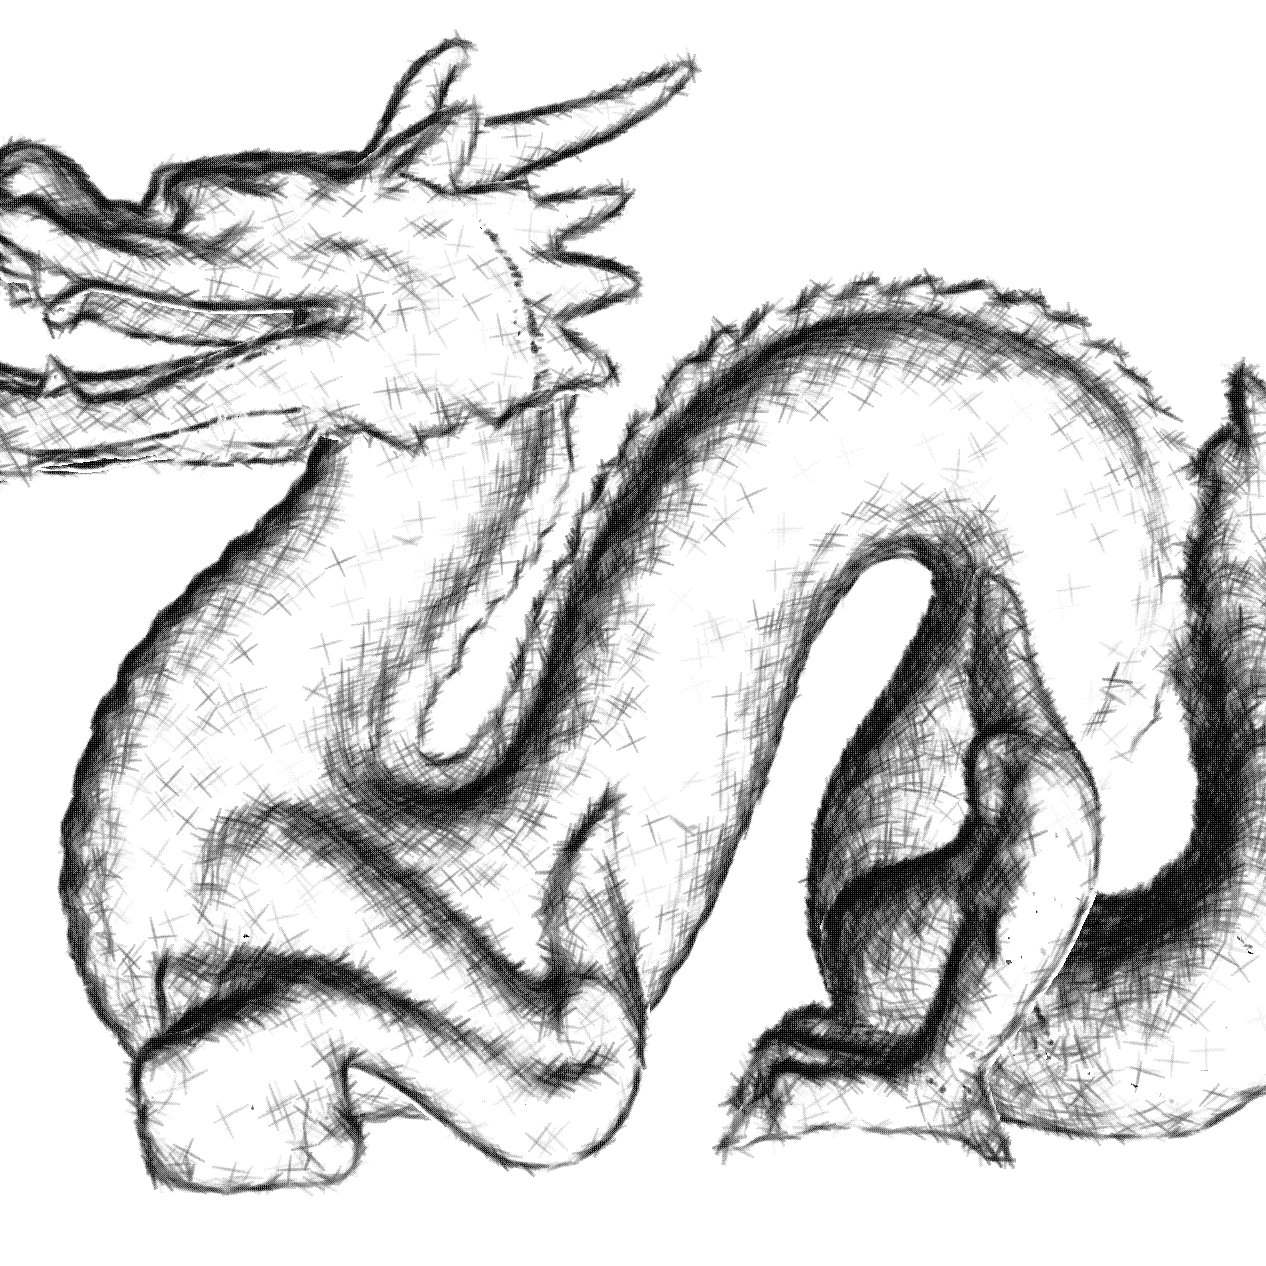
\includegraphics[width = \twffffp]{figures/dragon-final-v2-square}};
        \node[figRC, anchor = west](fig3) at ([xshift = \pfull] fig2.east)
            {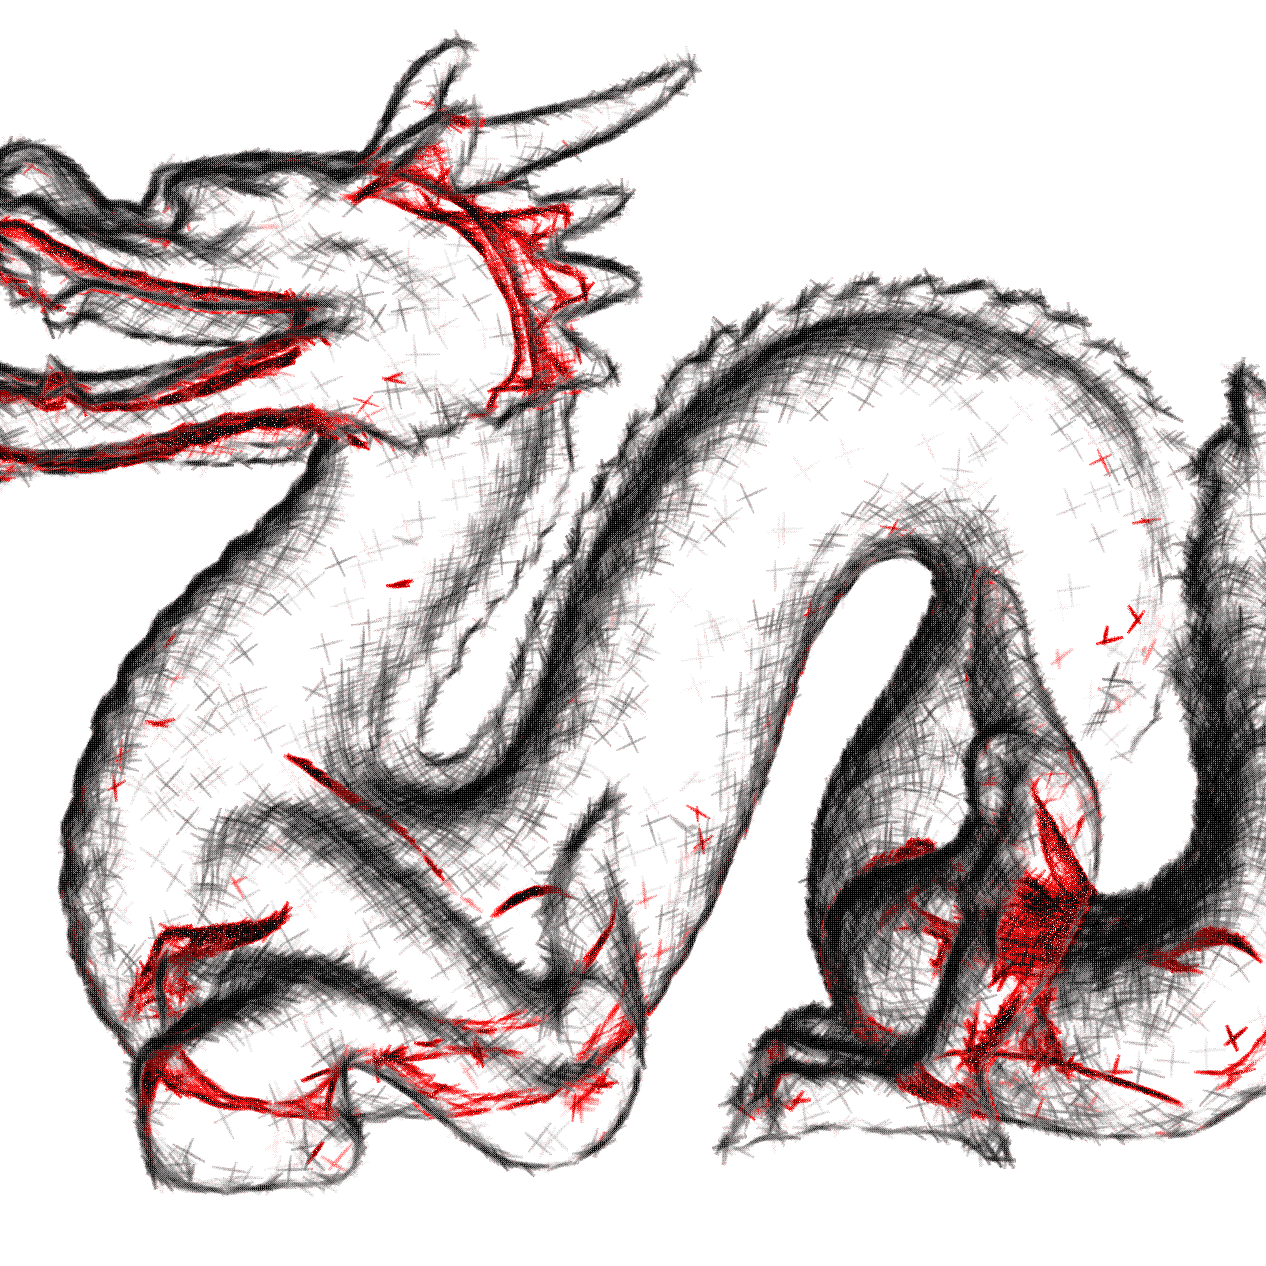
\includegraphics[width = \twffffp]{figures/dragon-depth-difference-v2-square}};
        % sub-captions/labels:
        \node[below = 0 and 0 of fig0, labelN](lab0){(a)~Naive Rendering};
        \node[below = 0 and 0 of fig1, labelN](lab1){(b)~Back Face enabled};
        \node[below = 0 and 0 of fig2, labelN](lab2){(c)~Depth Pass enabled};
        \node[below = 0 and 0 of fig3, labelN](lab3){(d)~Difference of (b) and (c)};
        % spies:
    \end{tikzpicture}
    %
    \caption{%
        The \emph{Stanford dragon} rendered as 3D point cloud (a)~without back face culling, (b)~with back face culling, and (c)~with an additional depth pass. 
        Points---or strokes---that are hidden due to the depth pass are highlighted in red in~(d).}
    \label{PCNPR:Fig:DepthPass}
\end{figure*}

In the depth pass, we render every point as a single circle and write only to the depth buffer.
With a sufficient point density and point size, these circles cover the whole surface, so in the following hatching pass, only lines in front of the surface get rendered.
Without any modifications however, the circles of the points at the front will cover the pencil strokes of nearby points. 
To avoid that problem, we add an offset to the polygons in the hatching pass, so the pencil strokes are slightly in front of their corresponding points from the depth pass~(\Cref{PCNPR:Fig:PolygonOffset} a).
Since the depth test needs to be activated in the drawing pass for this approach to work, we need to make sure nothing is written to the depth buffer in the hatching pass, otherwise the lines will cover each other instead of overlapping and thereby creating darker tones~(\Cref{PCNPR:Fig:PolygonOffset} b).

The size of the circles is also controllable via a parameter and needs to be adapted to achieve the desired result in the depth pass and to not cover too much or to little of the hatched lines.



\subsection{Enhancements}
\label{PCNPR:SubSec:Enhancements}
%
The approach described so far allows for decent results, though the following tweaks should be considered.


\paragraph{Alpha Modification.}
%
So far, we use the approach of probabilistic interpolation to create the impression of the surface being transparent.
However, for image regions with almost full transparency, this results in very few strong strokes on an otherwise clear part of the surface, when in an actual pencil sketch, you would also adjust the pressure of the pencil to modify the transparency of the strokes themselves.
That is why we adjust the alpha value of the generated pencil stroke proportional to the alpha value from the X-Toon texture.
Also, even in parts with similar lighting, not every stroke is applied with exactly the same pressure. To account for that, we apply some randomness on the final alpha value.

\paragraph{Interpolation of Cross \& Parallel Hatches.}
\label{PCNPR:Sec:CrossParallelInterpolation}
%
In addition to a decreased stroke strength, another technique to convey higher transparency is to use fewer lines by transitioning from cross hatching to parallel hatching.
We implement this approach by using the alpha value from the X-Toon texture as the probability for replacing a point with a cross instead of a line.
We multiply that probability by a parameter $h\in [0,1]$, allowing us to influence the proportion of cross-hatched to parallel-hatched points.
This parameter also makes it possible to create results that exclusively use parallel hatching.


\paragraph{Curvature-controlled Line-length.}
%
So far, we replace each point with equally long, straight lines.
Put together, they already create a good illustration of curved surfaces because the lines are short enough that they are a good approximation of the direction of the surface below them.
On areas of high curvature on the other hand, the surface direction changes faster. That means a line that is as long as the lines on low-curvature areas is not a good surface approximation anymore.
With curvature information at each point, we can align for that by decreasing the length of lines in high-curvature areas~(\Cref{PCNPR:Fig:Curvature}).
%
In addition to line length modification through curvature, we also modify the line length with a randomness factor to account for the differences in line length when drawing by hand.




\section{Results \& Discussion}
\label{PCNPR:Sec:ApplicationsAndDiscussion}
%
This section present and discusses various application examples achieved by using our art-directable rendering technique.


\paragraph{Application Examples.}
%
\Cref{PCNPR:Fig:MoreResults} shows an overview of different point cloud stylization variants obtained by our technique.
The variety covers a range from blueprint rendering, gray-scale charcoal and ballpoint pens to classic pencil drawing
or pointillism.
Our technique allows for modification of all provided stylization parameters and presents them interactively to 
support the demands of artists.


\paragraph{Performance Considerations.}
%
We tested the rendering performance of a prototypical implementation using three point clouds of different complexity ranging
from approx. 3.5 million points (LiDAR, Statue) over 5.7 million points to  11 million points (Angel statue, sampled 3D mesh). The first point cloud with 3.5 million points resulted in a frametime of about 30 milliseconds, with 5.7 million points we measured 60 milliseconds and for 11 million points we obtain a frametime of 100 milliseconds.
The performance test was conducted using an AMD Radeon 5700XT with 8 GB VRAM on a Ryzen 5 CPU with 3.6 GHz and 32 GB RAM
rendering at a viewport resolution of $2947 \times 1661$ pixels.
The run-time performance depends mainly on the geometric complexity of the 3D  scene and decreases approx. linearly with the number of points to process.
However, while a high point density is useful for the depth pass to avoid gaps between points it is 
not conducive to the overall visual quality of the hatching effect, \ie the generated strokes are hardly distinguishable.


\paragraph{Discussion.}
%
Due to the nature of point clouds, especially when created using consumer LiDAR scanners, outliers from the depth pass (remember, all points are used for this pass) sometimes cover strokes and might not be desired.
Similarly, the point cloud density is typically rather irregular, which sometimes leads to strokes bleeding from the background into the foreground.
Both effects can be mitigated by tweaking the polygon offset as well as the adjusting the point size within the depth pass.
Furthermore, these effects are not inherently wrong and are often also desirable for less dense point clouds.

The same applies for strokes which leave an object's expected silhouette or contour (over-shooting of strokes).
For us, this was mostly visually pleasing and also a welcome differentiator from image-based renderings.
There might be cases where this is not desired or not fitting a specific style though.
Since point clouds are never expected to be two manifold (\ie watertight or closed) and more often used for capturing open environments than for solid and closed objects, we render the mentioned drawbacks as non-problematic exceptions of our technique.
The distinctive styles can be easily achieved with only minor configurations within our art-directed parameterization and the technique can be implemented without exotic extension or groundbreaking graphics APIs.

\begin{figure*}[p] % requires figures-spec.tex
    %
    \begin{tikzpicture}[figNS, spy using outlines = {style = spyRC, magnification = 2.5, size = 20mm}]
        % graphics:
        % --- Bunnies!
        \node[figRC, anchor = east](fig0) at (0,0)
            {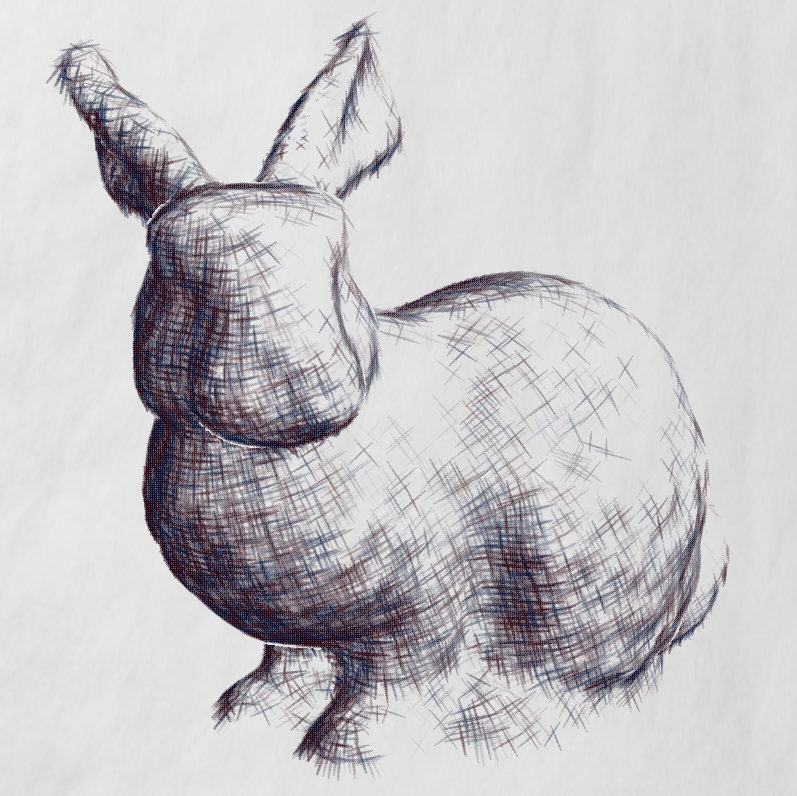
\includegraphics[width = \twfffp]{figures/results-bunny-1-v2}};
        \node[figRC, anchor = west](fig1) at ([xshift = \pfull] fig0.east) 
            {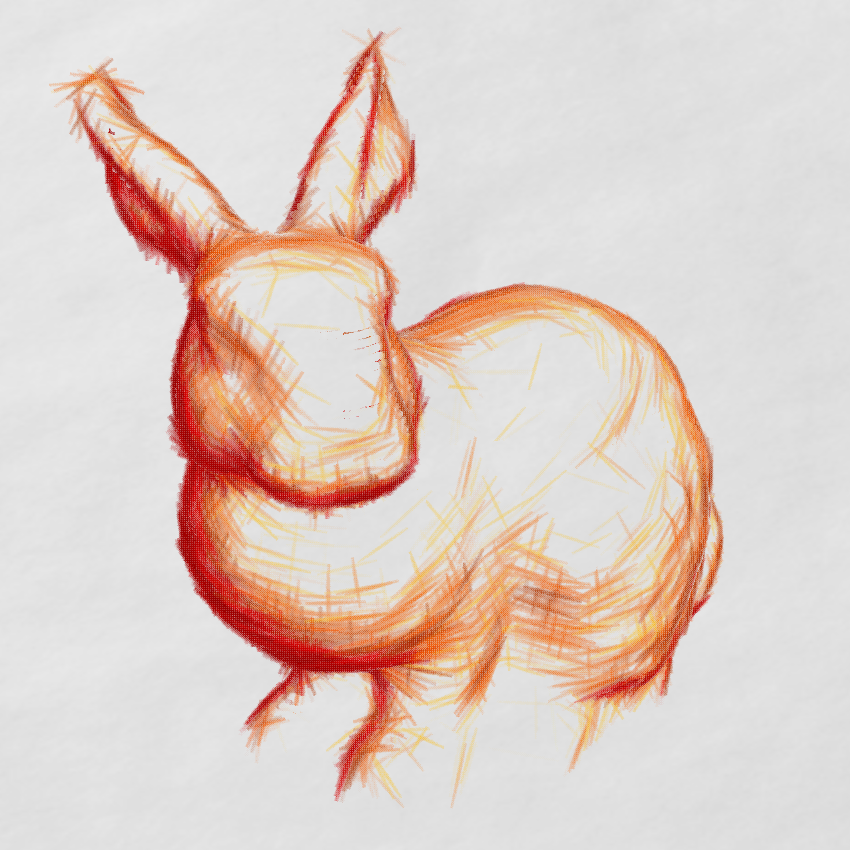
\includegraphics[width = \twfffp]{figures/results-bunny-2-v2}};
        \node[figRC, anchor = west](fig2) at ([xshift = \pfull] fig1.east)
            {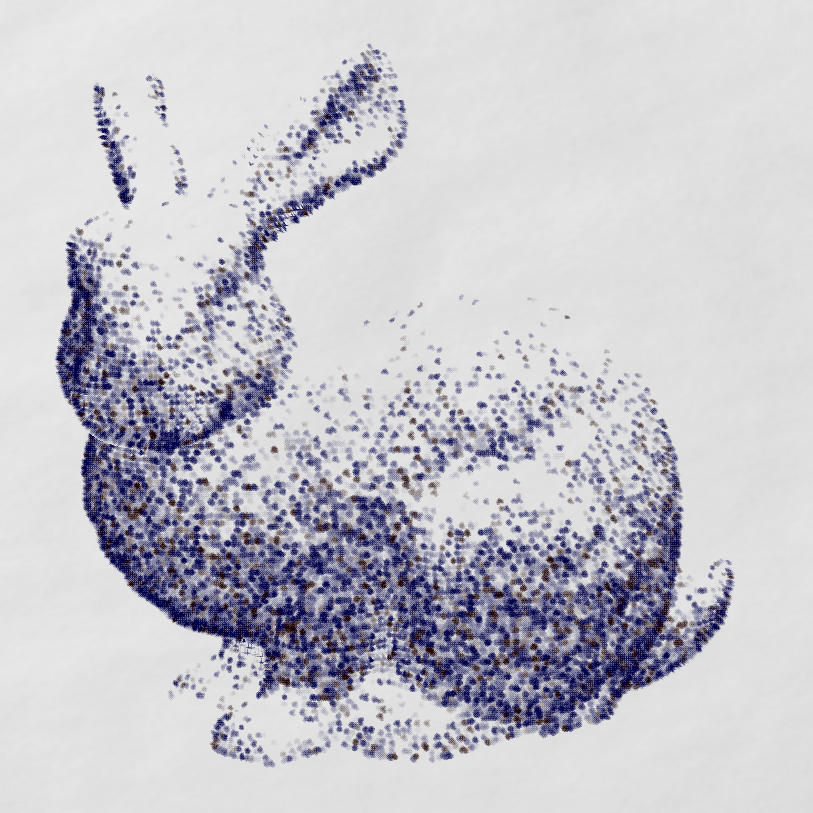
\includegraphics[width = \twfffp]{figures/results-bunny-7-v2}};
        % --- More Bunnies!
        \node[figRC, anchor = north](fig3) at ([yshift = -\pfull] fig0.south)
            {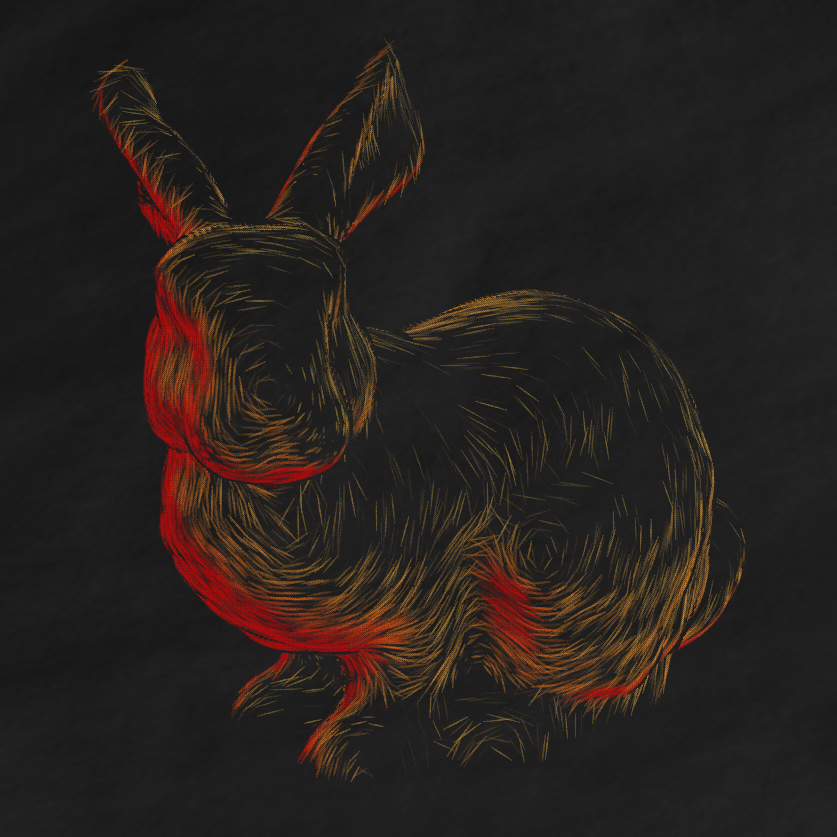
\includegraphics[width = \twfffp]{figures/results-bunny-4-v2}};
        \node[figRC, anchor = west](fig4) at ([xshift = \pfull] fig3.east)
            {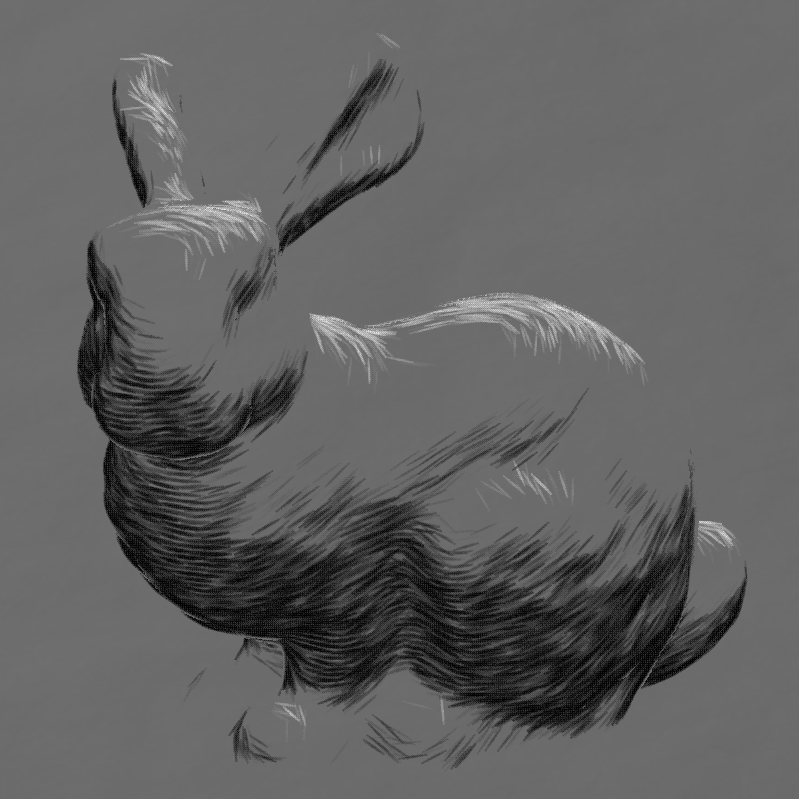
\includegraphics[width = \twfffp]{figures/results-bunny-5-v2}};
        \node[figRC, anchor = west](fig5) at ([xshift = \pfull] fig4.east)
            {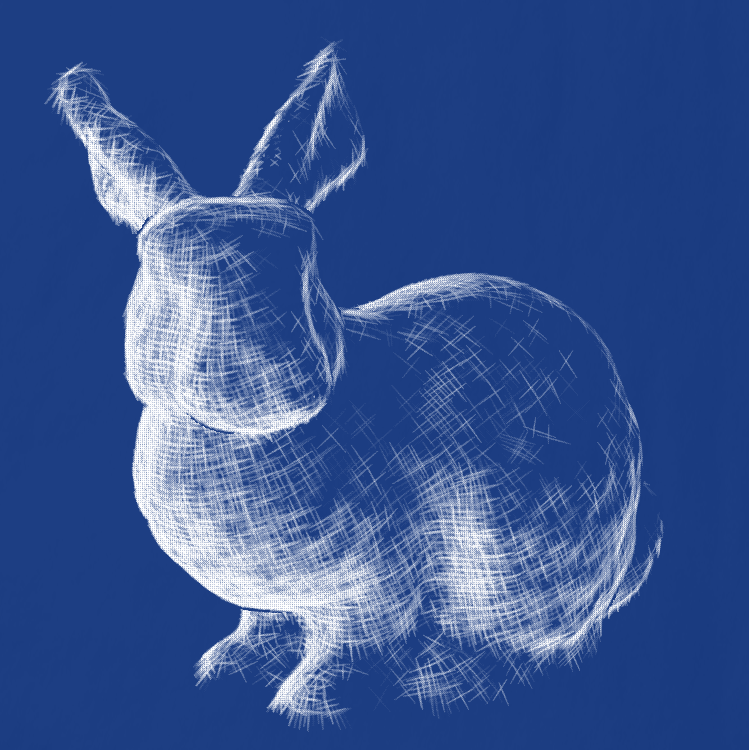
\includegraphics[width = \twfffp]{figures/results-bunny-8-v2}};
        %
        % --- Some Scans
         \node[figRC, anchor = north](fig6) at ([yshift = -\pfull] fig3.south)
            {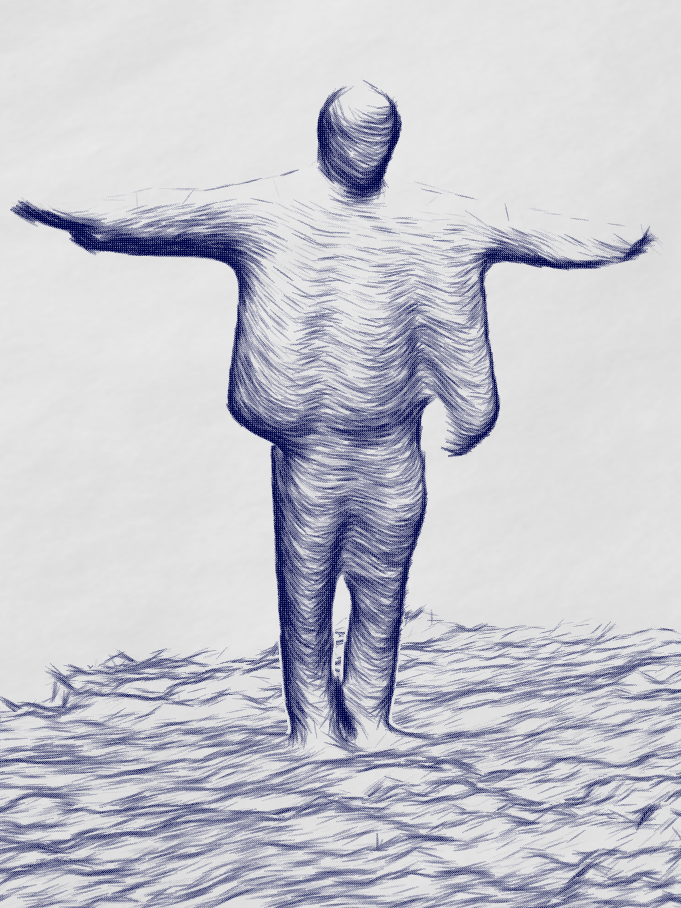
\includegraphics[width = \twfffp]{figures/results-scan-1-v2}};
        \node[figRC, anchor = west](fig7) at ([xshift = \pfull] fig6.east) 
            {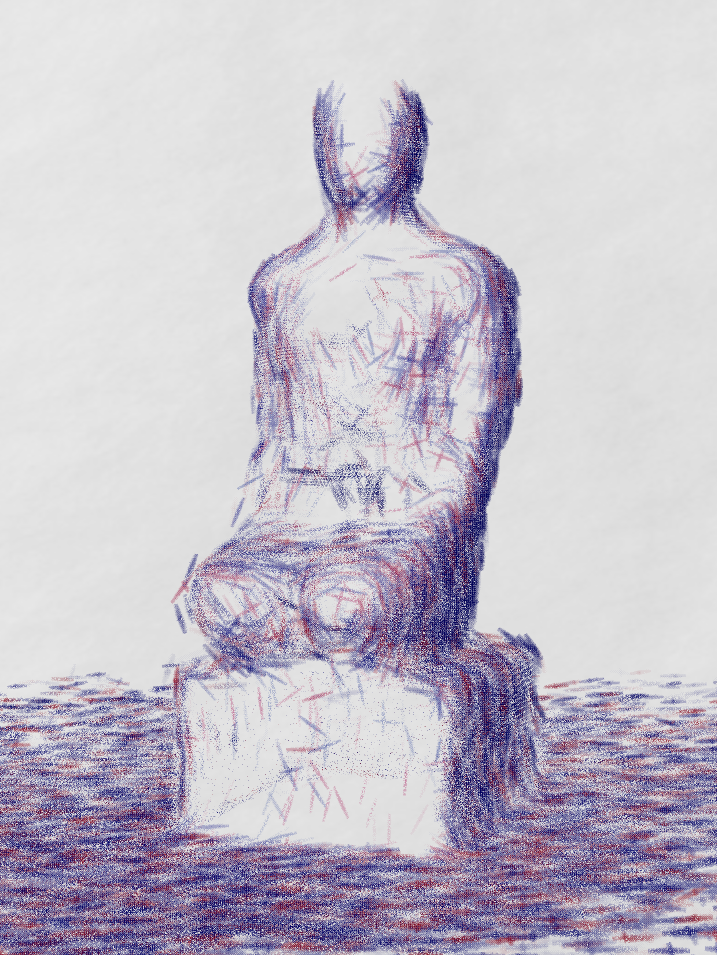
\includegraphics[width = \twfffp]{figures/results-scan-2-v2}};
        \node[figRC, anchor = west](fig8) at ([xshift = \pfull] fig7.east)
            {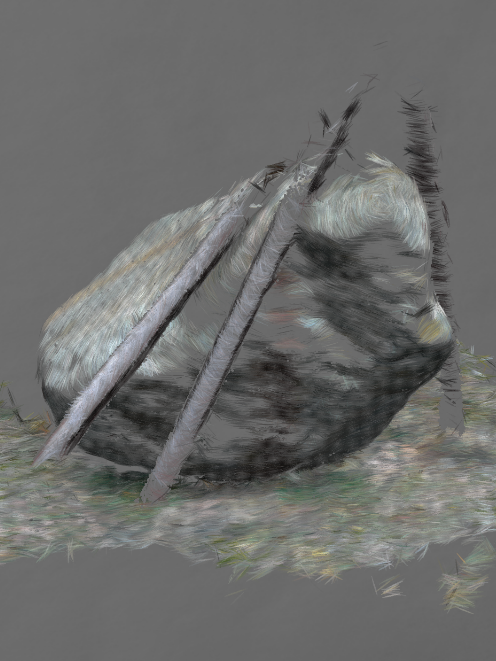
\includegraphics[width = \twfffp]{figures/results-scan-4-v2}};
        %
        % --- Some Meshes
         \node[figRC, anchor = north west](fig9) at ([yshift = -\pfull] fig6.south west)
            {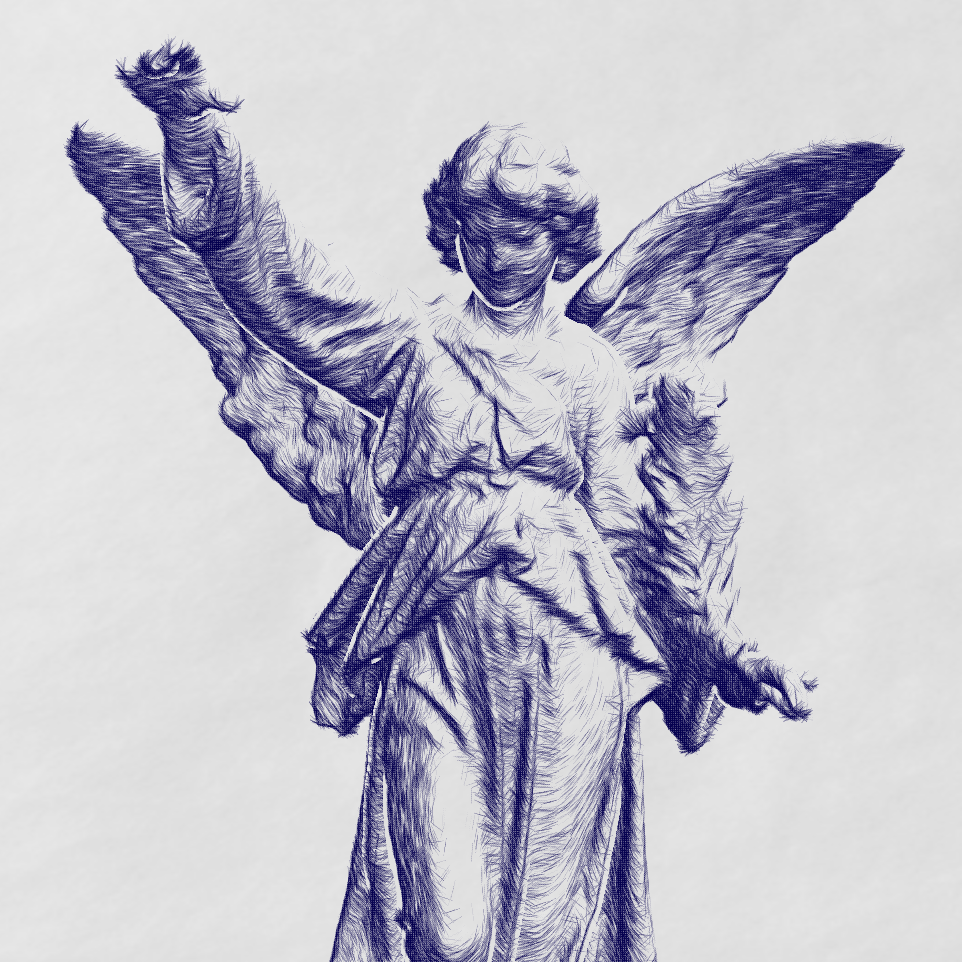
\includegraphics[width = \twffffp]{figures/results-mesh-1-v2}};
        \node[figRC, anchor = west](fig10) at ([xshift = \pfull] fig9.east) 
            {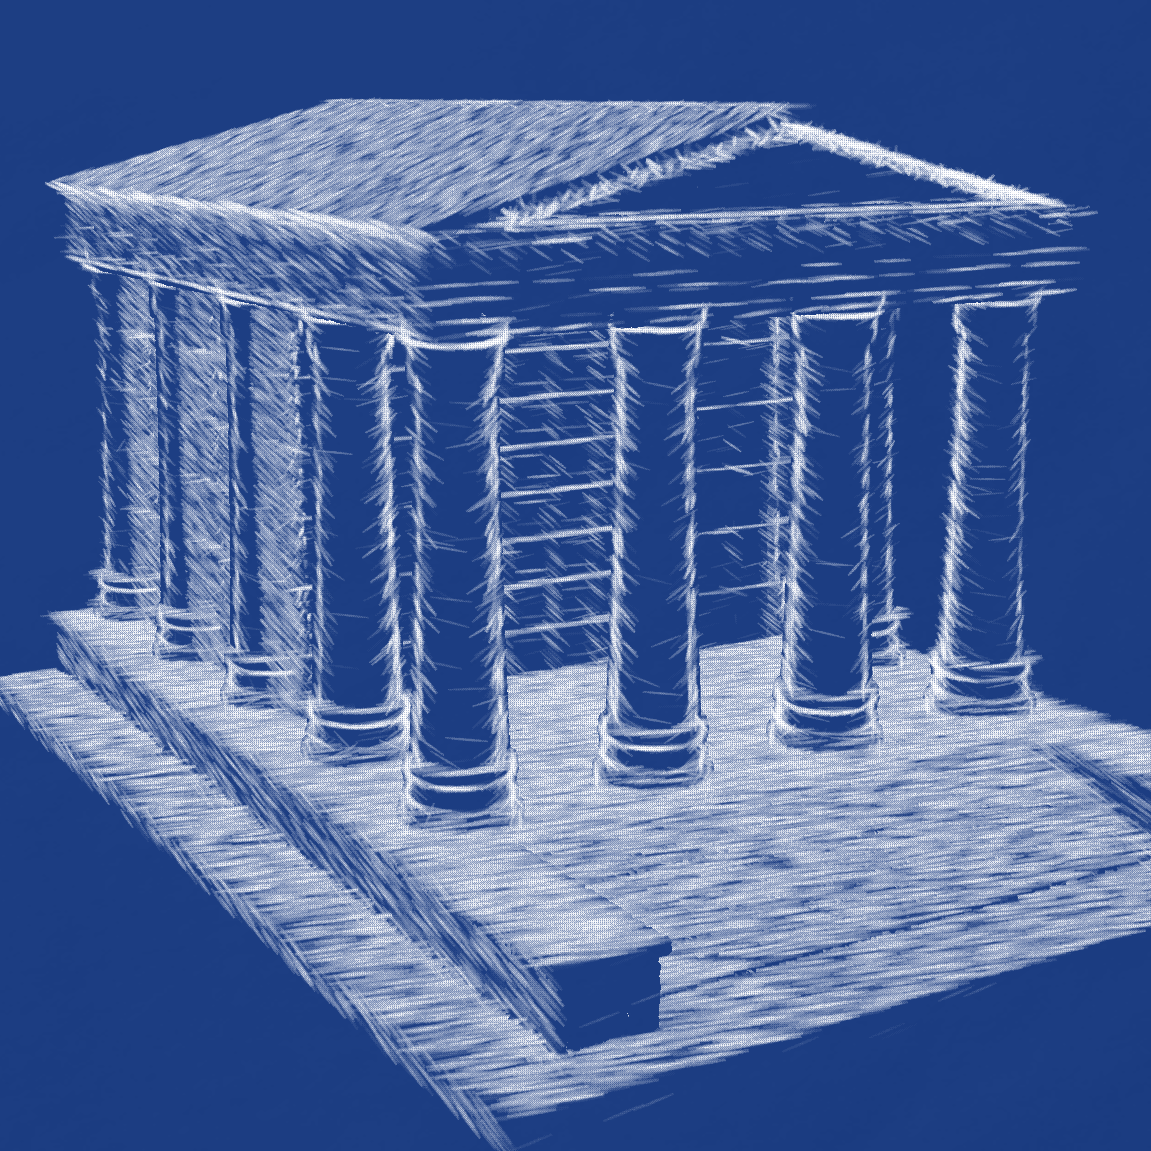
\includegraphics[width = \twffffp]{figures/results-mesh-2-v2}};
        \node[figRC, anchor = west](fig11) at ([xshift = \pfull] fig10.east)
            {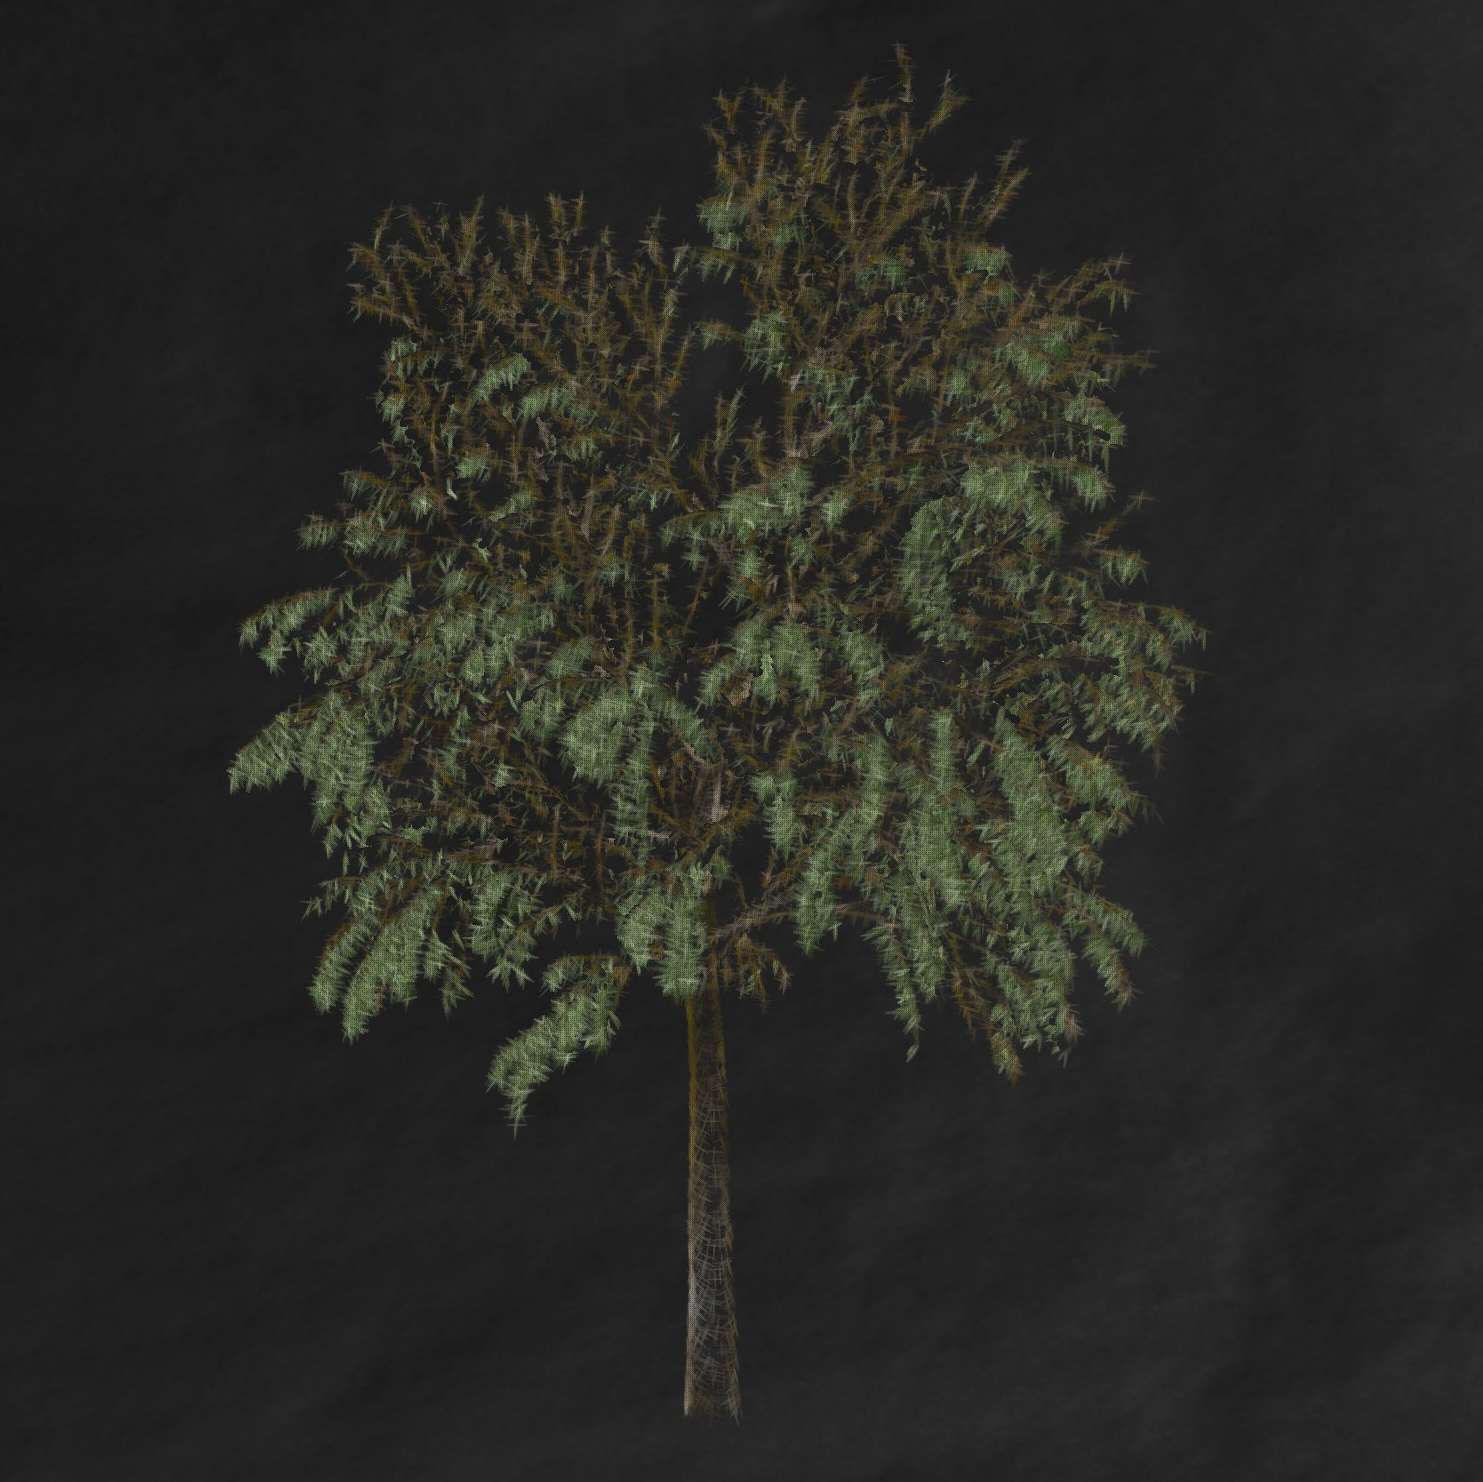
\includegraphics[width = \twffffp]{figures/results-mesh-3-v2}};
        \node[figRC, anchor = west](fig12) at ([xshift = \pfull] fig11.east)
            {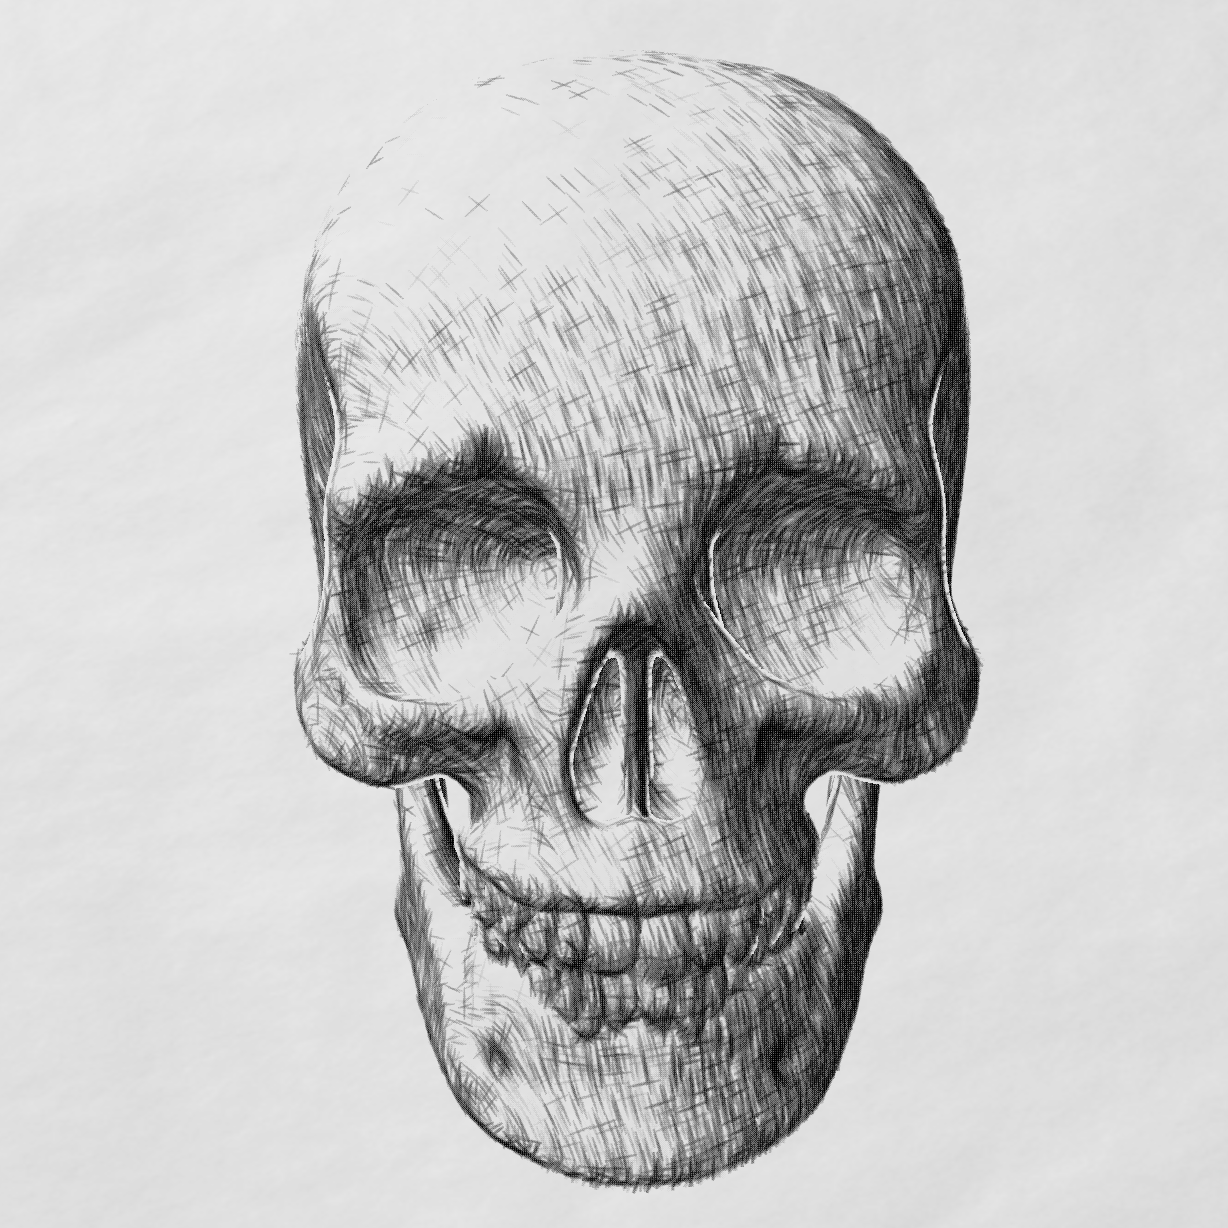
\includegraphics[width = \twffffp]{figures/results-mesh-4-v2}};
        % sub-captions/labels:
        \node[below left = 0 of fig0,  labelSW](lab0){(a)~Cross Hatched};
        \node[below left = 0 of fig1,  labelSW](lab0){(b)~Colorful Contour};
        \node[below left = 0 of fig2,  labelSW](lab0){(c)~Classic Pointillism};
        \node[below left = 0 of fig3,  labelSW](lab0){(d)~Two-Colored Dark};
        \node[below left = 0 of fig4,  labelSW](lab0){(e)~White and Black Chalk};
        \node[below left = 0 of fig5,  labelSW](lab0){(f)~Blueprint};
        % --- 
        \node[below left = 0 of fig6,  labelSW](lab0){(g)~iPad Scan, Hatched};
        \node[below left = 0 of fig7,  labelSW](lab0){(h)~iPad Scan, Cross Hatched};
        \node[below left = 0 of fig8,  labelSW](lab0){(i)~iPad Scan, Crayons};
        % --- 
        \node[below left = 0 of fig9,  labelSW](lab0){(j)~Statue};
        \node[below left = 0 of fig10, labelSW](lab0){(k)~Temple};
        \node[below left = 0 of fig11, labelSW](lab0){(l)~Tree with Leaves};        
        \node[below left = 0 of fig12, labelSW](lab0){(m)~Skull};
        % spies:
        \spy on ($(fig0.center)+( -8mm, +12mm)$) in node at ($(fig0.center)+(+14mm,+14mm)$);
        \spy on ($(fig1.center)+( -8mm, +12mm)$) in node at ($(fig1.center)+(+14mm,+14mm)$);
        \spy on ($(fig2.center)+(-12mm,  +8mm)$) in node at ($(fig2.center)+(+14mm,+14mm)$);
        \spy on ($(fig3.center)+( -8mm, +12mm)$) in node at ($(fig3.center)+(+14mm,+14mm)$);
        \spy on ($(fig4.center)+( -8mm, +12mm)$) in node at ($(fig4.center)+(+14mm,+14mm)$);
        \spy on ($(fig5.center)+( -8mm, +12mm)$) in node at ($(fig5.center)+(+14mm,+14mm)$);
        % ---
        \spy on ($(fig6.center)+( -4mm, -16mm)$) in node at ($(fig6.center)+(+14mm,-18mm)$);
        \spy on ($(fig7.center)+(-10mm,  -8mm)$) in node at ($(fig7.center)+(+14mm,-18mm)$);
        \spy on ($(fig8.center)+( -8mm,   0mm)$) in node at ($(fig8.center)+(+14mm,-18mm)$);
        % ---
        \spy on ($(fig11.center)+(-1mm,  -6mm)$) in node at ($(fig11.center)+(+18mm,+6mm)$);
    \end{tikzpicture}
    %
    \caption{%
        Various results of our NPR rendering-technique. A point cloud scan of the \emph{Stanford bunny} was used in (a) to (f).
        The point clouds in (g) to (i) have are actual point clouds captured using an iPad.
        In (j) to (m) the points are sampled from 3D polygonal meshes and rendered using our NPR technique.
        All results are captured from our C++ implementation, rendered interactively and in real-time ($60\textrm{Hz}+$ in Full-HD and QHD) with a temporal coherence not possible using image-based approaches.
        Meshes used for (j) and (k) are licensed under \emph{CC Attribution} and have been created by \emph{noe-3d.at}~(\href{https://sketchfab.com/3d-models/grabfigur-cfec3a9d71db42978d4a377a0e8f1154}{sketchfab.com/3d-models/grabfigur-cfec3a9d71db42978d4a377a0e8f1154}) and \emph{Robin Butler}~(\href{https://sketchfab.com/3d-models/roman-temple-f5efe108fb19419ab985ef69d1762839}{sketchfab.com/3d-models/roman-temple-f5efe108fb19419ab985ef69d1762839}) respectively.}
    \label{PCNPR:Fig:MoreResults}
\end{figure*}




\section{\texorpdfstring{\uppercase{Conclusions}}{Conclusions}}%
\label{PCNPR:Sec:Conclusions}
%
This paper presents a real-time non-photorealistic rendering technique for art-directed hatches of 3D point clouds.
By extending the X-Toon approach of Barla \etal, it facilitates various configurations yielding different stylization results for potentially massive 3D point clouds that are obtained by \ac{LiDAR} acquisition or sampling polygonal 3D meshes. 
%
The current state provides basis to develop and apply more advanced stylization techniques for 3D point clouds.
For example, to synthesize more sophisticated stylized renderings, our technique can be extended to support outlines~\cite{Rosenthal2008} or even suggestive contours~\cite{ProencaJS2008} using the derived curvature information~\cite{Merigot2009,Lu2020}. 
Further, level-of-detail approaches for geometry generation stage can be implemented enabling seamless 
level-of-abstraction transitions~\cite{SD14}.
Furthermore, the depth pass could be improved by using oriented point splats~\cite{Anjos2018}.




\section*{\uppercase{Acknowledgments}}
%
We thank the anonymous reviewers for their valuable feedback. 
This work was partially funded by the \ac{BMBF} through grants 01IS18092 (\enquote{mdViPro}) and 01IS19006 (\enquote{KI-LAB-ITSE}).




{
\small%
\bibliographystyle{apalike}
\bibliography{pc-npr}}


\begin{acronym}
\acro{AABB}{Axis-aligned Bounding Box}
\acro{adaIN}{adaptive Instance Normalization}
\acro{AoS}{Array-of-Structures}
\acro{API}{Application Programming Interface}

\acro{B2C}{Business-to-Customer}
\acro{B2B}{Business-to-Business}
\acro{BMBF}{German Federal Ministry of Education and Research}
\acro{CAS}{Content Analysis Service}
\acro{CIN}{Conditional Instance Normalization}
\acro{CMS}{Content Moderation Service}
\acro{CNN}{Convolutional Neural Network}
\acro{CPU}{Central Processing Unit}
\acro{CS}{Compute Shader}
\acro{CSS}{Cascading Style Sheets}


\acro{DBS}{Density-Based Sampling}
\acro{DCC}{Digital Content Creation}
\acro{DOM}{Document Object Model}
\acro{DRM}{Digital Rights Management}

\acro{EC2}{Elastic Compute Cloud}

\acro{FHD}{Full High Definition}
\acro{FPS}{Frames-per-Second}

\acro{GCM}{Google Cloud Messaging}
\acro{GPU}{Graphics Processing Unit}

\acro{HD}{High Definition}
\acro{HDR}{High Dynamic Range}
\acro{HTML}{Hyper Text Markup Language}

\acro{IAS}{Image Abstraction Service}

\acro{JPEG}{Joint Photographic Experts Group}
\acro{JS}{JavaScript}

\acro{LiDAR}{Light Detection And Ranging}

\acro{ML}{Machine Learning}
\acro{Mpix}{Megapixel}

\acro{NPR}{Non-Photorealistic Rendering}
\acro{NSFW}{Not Safe For Work}
\acro{NST}{Neural Style Transfer}

\acro{OGC}{Open Geospatial Consortium}
\acro{ONNX}{Open Neural Network Exchange}
\acro{OpenGL}{Open Graphics Library}
\acro{OS}{Operating System}

\acro{PBS}{Primitive-Based Sampling}
\acro{PC}{point cloud}

\acro{QHD}{Quad High Definition}

\acro{RAM}{Random Access Memory}
\acro{REST}{Representational State Transfer}

\acro{SoA}{Structure-of-Arrays}
\acro{SSBO}{Shader Storage Buffer Object}
\acro{SSD}{Single Shot Detector}

\acro{TOS}{Terms of Service}

\acro{UGC}{User-Generated Content}
\acro{UI}{User Interface}
\acro{URL}{Unified Resource Locator}

\acro{VBO}{Vertex Buffer Object}
\acro{VBS}{Vertex-\textbf{b}ased Sampling}
\acro{vCPU}{virtual CPU}
\acro{VRAM}{Video Random Access Memory}

\acro{W3C}{World Wide Web Consortium}
\acro{WebGL}{Web Graphics Library}

\end{acronym}

\end{document}
